%----------------------------------------------------------------
%
%  File    :  survey.tex
%
%  Author  :  Keith Andrews, ISDS, TU Graz, Austria
%
%  Created :  24 Mar 2010
%
%  Changed :  22 Jan 2021
%
%----------------------------------------------------------------


\documentclass[11pt,onecolumn,twoside]{report}

\usepackage[
  a4paper,
  twoside,
  top=5mm,                % top margin
  bottom=7mm,             % bottom margin
  inner=20mm,             % inner margin (next to binding)
  outer=20mm,             % outer margin (opposite binding)
  bindingoffset=10mm,     % on binding side
  includeheadfoot,        % include head(er) and foot(er)
  headheight=10mm,        % height of header
  headsep=15mm,           % sep between header and text body
  footskip=15mm,          % sep between body and baseline of footer
  footnotesep = 10mm plus 2mm minus 0mm  % bottom of body to top of footnote
]{geometry}
% A4 paper is w=210m, h=297mm


\newcommand{\thistitle}{Checking Web Accessibility}  % title
% \newcommand{\thissubject}{Guidelines for Writing a Survey Paper in Computer Science}  % subject
\newcommand{\thissubject}{}  % leave empty for no subject
\newcommand{\thisauthor}{Ožbej Golob, Alexander Thien, Olli-Pekka Riikola, Robin Karlsson}          % author
% \newcommand{\thisauthor}{Keith Andrews, Tom Black, and Harry White}      % multiple authors
\newcommand{\thiskeywords}{web accessibility, screen readers, text-only browsers, accessibilty audit tools}   % keywords

\newcommand{\thisdate}{10 Nov 2021}  % date of this version
\newcommand{\thisyear}{2021}         % year of this version




\newcommand{\fullh}{24cm}         % height of figures for 1 per page
\newcommand{\halfh}{9.5cm}        % height of figures for 2 per page
\newcommand{\thirdh}{6cm}         % height of figures for 3 per page


\setlength{\parindent}{1em}       % less indentation
\setlength{\parskip}{5pt plus 1pt minus 1pt}  % space before a paragraph


% \tolerance is set by LaTeX to 200
% \sloppy sets \tolerance = 9999
% which allows LaTeX more tolerance in adding word spacing

% \sloppy
% \fussy
% \tolerance = 1000

\tolerance=400 
% makes some lines with lots of white space, but      
% tends to prevent words from sticking out in the margin



\setcounter{tocdepth}{3}        % lowest section level entered in ToC
\setcounter{secnumdepth}{3}     % lowest section level still numbered




\usepackage[T1]{fontenc}        % 8-bit output chars (must be before inputenx)
\usepackage[utf8]{inputenx}     % input char encoding

\usepackage[english,austrian,british]{babel}

\usepackage{newtxtext}          % newer times fonts
\usepackage{newtxmath}

\usepackage{relsize}            % relative font sizes \smaller \larger
\usepackage{float}              % H for float placement
\usepackage{setspace}           % line spacing

\usepackage{textcomp}           % symbols such as \texttimes and \texteuro
\usepackage{latexsym}
\usepackage{fontawesome}        % fontawesome symbols

\usepackage{siunitx}            % prettier number formatting
\sisetup{%
  group-separator={,},
}
\usepackage[super]{nth}         % 1st, 2nd, 3rd, etc.

\usepackage{xspace}
\usepackage{xstring}            % string manipulation macros
\usepackage{xparse}             % commands with optional arguments
\usepackage{etoolbox}           % for \newrobustcmd
\usepackage{makecmds}           % for \makecommand
\usepackage{calc}               % for math calculations

\usepackage[svgnames,table,xcdraw]{xcolor}
\definecolor{darkgreen}{rgb}{0.0,0.2,0.0}
\definecolor{darkblue}{rgb}{0.0,0.0,0.2}
\definecolor{darkred}{rgb}{0.2,0.0,0.0}
\definecolor{verylightgrey}{gray}{0.95}
\definecolor{lightgrey}{gray}{0.9}
\definecolor{grey}{gray}{0.7}
\definecolor{black}{gray}{0.0}

\definecolor{tableheadercolour}{gray}{0.8}
\definecolor{tablerowcolour}{gray}{0.93}



\usepackage{longtable}
\usepackage{multirow}
\usepackage{tabularx}

% Define some new column types for tables:
% like X but flushleft (= raggedright) rather than justified
\newcolumntype{Y}{>{\raggedright\arraybackslash}X}
% a p column but flushleft (= raggedright) rather than justified
\newcolumntype{L}[1]{>{\raggedright\arraybackslash}p{#1}}
% a p column but flushright (= raggedleft) rather than justified
\newcolumntype{R}[1]{>{\raggedleft\arraybackslash}p{#1}}


\usepackage{booktabs}           % nicer tables

\newcommand{\tablestretch}
{\renewcommand{\arraystretch}{1.20}}  % spacing between table rows




\usepackage{verbdef}            % define robust verb strings
\usepackage{verbatim}
\usepackage{comment}



% better lists
\usepackage{enumitem}

\setlist{
  topsep=0pt,
  partopsep=0pt,
  parsep=0.6ex,
  itemsep=1.2ex,
  left=\parindent .. 2\parindent,    % bullet .. start ot text
}

\setlist[description]{
  style=sameline,
}




\usepackage{listings}                 % for listings of source code

\makeatletter
\newlength{\numwidth}%
\setlength{\numwidth}{\widthof{\normalfont{\lst@numberstyle{99}}}}% Up to 2-digit (99) line numbers
\def\lst@PlaceNumber{%
  \makebox[\numwidth+1em][l]{%
    \makebox[\numwidth][r]{\normalfont\lst@numberstyle{\thelstnumber}}%
  }%
}
\makeatother

% lstset strategy: define defaults here for
% all non-floating (displayed) listings
% floated listings override these settings later

\lstset{                              % set parameters for listings
  floatplacement=tp,                  % default float placement
  numberbychapter,
  inputencoding=utf8,
  language=,                          % empty = plain text
  basicstyle=\small\ttfamily,
  tabsize=2,
  xleftmargin=2\parindent,
  xrightmargin=2\parindent,
  frame=none,
  framexleftmargin=0mm,
  rulesepcolor=\color{verylightgrey},
  numbers=none,
  numberstyle=\scriptsize,
  numbersep=2ex,
  breaklines,
  showtabs=false,
  showspaces=false,
  showstringspaces=false,
  keywordstyle=\color{black},
  commentstyle=\color{SteelBlue},
  identifierstyle=,
  stringstyle=,
  captionpos=b,
  abovecaptionskip=\abovecaptionskip,
  belowcaptionskip=\belowcaptionskip,
  extendedchars=true,           % listings usually only support 7-bit ascii chars
  literate=%                    % map some one-byte utf8 chars for use in listings
%    { }{{~}}1                   % non-breaking space
    {©}{{\textcopyright}}1
    {€}{{\texteuro}}1
    {Ö}{{\"O}}1
    {Ä}{{\"A}}1
    {Ü}{{\"U}}1
    {ß}{{\ss}}1
    {ö}{{\"o}}1
    {ä}{{\"a}}1
    {ü}{{\"u}}1,
}


\lstdefinelanguage{biblatex}   % based on biblatex v 2.7a from 2013-07-14
{
  keywords={%
    @article,@book,@mvbook,@inbook,@bookinbook,@suppbook,%
    @booklet,@collection,@mvcollection,@incollection,@suppcollection,%
    @manual,@misc,@online,@patent,@periodical,@suppperiodical,%
    @proceedings,@mvproceedings,@inproceedings,@reference,@mvreference,%
    @inreference,@report,@set,@thesis,@unpublished,@xdata,%
    @conference,@electronic,@mastersthesis,@phdthesis,@techreport,@www,%
    @artwork,@audio,@bibnote,@commentary,@image,@jurisdiction,@legislation,%
    @legal,@letter,@movie,@music,@performance,@review,@software,%
    @standard,@video%
  },
  sensitive=false,
  comment=[l][\itshape]{@comment},
  morecomment=[l]{\%},
}

\lstdefinelanguage{CSS}
{
  alsoletter={-},
  morekeywords={%
  color,background,background-color,margin,padding,font,
  font-family,weight,%
  display,position,top,left,right,bottom,list,%
  style,border,size,white,space,min,width%
  },
  sensitive=false,
  morecomment=[l]{//},
  morecomment=[s]{/*}{*/},
  morestring=[b]",
}





\usepackage[compact,nobottomtitles,pagestyles,explicit]{titlesec}
% when using explicit, must explicitly include #1 for titlename

% nobottomtitles
% move section headings close to page bottom to next page
\renewcommand{\bottomtitlespace}{2cm}

% \chaptermark sets the value of \chaptertitle for later
% \@chapapp is defined as \chaptername outside the appendix,
% and as \appendixname within the appendix.
\makeatletter
\titleformat{\chapter}
[display]                                            % shape
{\chaptermark{\thechapter~~#1}\sffamily\bfseries}    % format
{\huge\@chapapp\ \thechapter}                        % label
{4ex}                                                % sep
{\Huge#1}                                            % before-code
\makeatother

\titleformat{name=\chapter,numberless}
[block]                                              % shape
{\chaptermark{#1}\sffamily\bfseries}                 % format
{}                                                   % label
{0ex}                                                % sep
{\Huge#1}                                            % before-code

\titleformat{\section}
{\normalfont\Large\sffamily\bfseries}{\thesection}{0.8em}{#1}

\titleformat{\subsection}
{\normalfont\large\sffamily\bfseries}{\thesubsection}{0.8em}{#1}

\titleformat{\subsubsection}
{\normalfont\normalsize\sffamily\bfseries}{\thesubsubsection}{0.8em}{#1}

\titleformat{\paragraph}[runin]
{\normalfont\normalsize\sffamily\bfseries}{\theparagraph}{0.8em}{#1}

\titleformat{\subparagraph}[runin]
{\normalfont\normalsize\sffamily\bfseries}{\thesubparagraph}{0.8em}{#1}


% vertical spacing before and after section titles
\titlespacing*{\section}
{0pt}{3.5ex plus 0.5ex minus 0.5ex}{0ex plus 0ex minus 0.2ex}

\titlespacing*{\subsection}
{0pt}{2.5ex plus 0.5ex minus 0.5ex}{0ex plus 0ex minus 0.2ex}

\titlespacing*{\subsubsection}
{0pt}{2ex plus 0.5ex minus 0.5ex}{0ex plus 0ex minus 0.2ex}


% define page headings how I want them

\newpagestyle{main}[\small]{
% \addtolength\headheight{6.7pt}
% \headrule
\sethead%
[{\parbox[t]{0.3\textwidth}%                    % even left
  {\sffamily\thepage}}]
[]%                                             % even centre
[{\parbox[t]{0.6\textwidth}%                    % even right
  {\raggedleft\sffamily\chaptertitle}}]
{{\parbox[t]{0.6\textwidth}%                    % odd left
  {\sffamily\sectiontitle}}}%
{}%                                             % odd centre
{{\parbox[t]{0.3\textwidth}%                    % odd right
  {\raggedleft\sffamily\thepage}}}
}




\usepackage{titletoc}

% \contentsmargin{2.55em}

\titlecontents{chapter}%
[1.5em]%                         % left indent to entry text
{\addvspace{1em}\bfseries}%      % above-code per entry
{\contentslabel{1.5em}}%         % format for numbered entry
{\hspace*{-1.5em}}%              % format for unnumbered entry
{\hfill\contentspage}%           % [no dots] and page num per entry


% Note: \dottedcontents is short form of \titlecontents

\dottedcontents{section}%
[3.8em]%                         % left indent to entry text = 1.5 + 2.3
{}%                              % above-code per entry
{2.3em}%                         % label width
{1pc}%                           % space around the dots

\dottedcontents{subsection}%
[7.4em]%                         % left indent to entry text = 3.8 + 3.6
{}%                              % above-code per entry
{3.6em}%                         % label width
{1pc}%                           % space around the dots


\dottedcontents{figure}%         % LoF entries
[3.0em]%                         % left indent to entry text = 3.8 + 3.6
{}%                              % above-code per entry
{3.0em}%                         % label width
{1pc}%                           % space around the dots

\dottedcontents{table}%          % LoT entries
[3.0em]%                         % left indent to entry text = 3.8 + 3.6
{}%                              % above-code per entry
{3.0em}%                         % label width
{1pc}%                           % space around the dots



% List of Listings is unknown to titletoc, define here

% Add extra per-chapter space to LoL to mimic LoF and LoT
% (requires package etoolbox)
\makeatletter
\patchcmd{\@chapter}% <cmd>
  {\addtocontents}% <search>
  {\addtocontents{lol}{\protect\addvspace{10\p@}}% add per-chapter space
   \addtocontents}% <replace>
  {}{}% <success><failure>
\makeatother

% Configure LoL to mimic LoF and LoT
\contentsuse{lstlisting}{lol}

\titlecontents{lstlisting}%
[3.0em]%                              % left indent
{\addvspace{1.5mm}}%                  % above-code per entry
{\contentslabel{3.0em}}%              % format for numbered entry
{\hspace*{-3.0em}}%                   % format for unnumbered entry
{\titlerule*[1pc]{.} \contentspage}%  % dots and page num per entry
[]%                                   % below-code per entry

\renewcommand{\lstlistlistingname}{List of Listings}






% sensible settings for floats

\setlength{\textfloatsep}{9mm plus 2mm minus 2mm}
\setlength{\floatsep}{9mm plus 2mm minus 2mm}
\setlength{\intextsep}{9mm plus 2mm minus 2mm}

\setlength{\dbltextfloatsep}{9mm plus 2mm minus 2mm}
\setlength{\dblfloatsep}{9mm plus 2mm minus 2mm}

\setlength{\abovecaptionskip}{4mm plus 2mm minus 1mm}
\setlength{\belowcaptionskip}{2mm plus 1mm minus 1mm}


% See http://www-rohan.sdsu.edu/~aty/bibliog/latex/floats.html
% See https://robjhyndman.com/hyndsight/latex-floats/

\setcounter{topnumber}{2}               % max num floats at top of page
\setcounter{dbltopnumber}{2}            % max num floats on 2col page
\setcounter{bottomnumber}{2}            % max num floats at bottom of page
\setcounter{totalnumber}{4}             % max num floats on a page

\renewcommand{\topfraction}{0.8}        % max fraction of floats at top
\renewcommand{\dbltopfraction}{0.9}     % max fraction of floats at top 2col
\renewcommand{\bottomfraction}{0.8}     % max fraction of floats at bottom
\renewcommand{\textfraction}{0.2}       % min fraction of text

% only for entirely float pages:
\renewcommand{\floatpagefraction}{0.7}      % min page fraction having floats
\renewcommand{\dblfloatpagefraction}{0.7}   % min 2col page fraction having floats


% \usepackage[section,above,below]{placeins}  % keep floats to their own section




% use caption and subfig (caption2 and subfigure are now obsolete)

\usepackage[
  position=bottom,
  margin=1cm,
  font=small,
  labelfont={bf,sf},
  format=plain,
  indention=5mm,
  aboveskip=4mm,
  belowskip=0mm,
]{caption,subfig}

\captionsetup[subfigure]{
  margin=0pt,
  parskip=0pt,
  indention=5mm,
  farskip=4mm,            % skip above subfig (assuming captions at bottom)
  captionskip=2mm,        % skip between subfig and subcaption
}




\usepackage[short]{datetime}   % load datetime *after* babel, requires fmtcount
% \newdateformat{britdate}{%
% \ordinaldate{\THEDAY} \,\monthname[\THEMONTH] \THEYEAR
% }
\newdateformat{unixdate}{%
\twodigit{\THEDAY}~\shortmonthname[\THEMONTH]~\THEYEAR
}



\usepackage[
  autostyle=true,          % adapt quote style to current language
  english=british,         % british english as default
  threshold=1,             % set block quotations >1 line in display mode
  maxlevel=4,              % max nesting level
]{csquotes}

\usepackage[
  indentfirst=false,
  vskip=0pt,               % by default would be \topsep + \partopsep.
]{quoting}

% tell csquotes to use quoting environment
% for \displayquote and \blockquote
\SetBlockEnvironment{quoting}

% if cite is issued by a csquote command
\renewcommand{\mkcitation}[1]{\space#1}

% I prefer double quotes as outer
\DeclareQuoteStyle{keithbritish}%  [variant]{style}
  {\textquotedblleft}%                      opening outer mark
  {\textquotedblright}%                     closing outer mark
  [0.05em]%
  {\textquoteleft}%                         opening inner mark
  {\textquoteright}%                        closing inner mark

\ExecuteQuoteOptions{style=keithbritish}





\usepackage[
  backend=biber,
%  style=ext-authoryear-comp,   % defined in biblatex-ext package
  style=ext-authoryear,        % defined in biblatex-ext package
  sorting=nyt,
  useprefix,                   % van and von are part of second name
  mergedate=false,             % only for authoryear style
  dashed=false,                % only for authoryear style
  abbreviate=false,
  maxcitenames=2,              % if > 2 authors,
  mincitenames=1,              % use first 1 then et al
  maxbibnames=99,              % if > 99 authors,
  minbibnames=6,               % use first 6 then et al
  uniquelist=minyear,
  uniquename=init,
  hyperref=true,
  backref=true,
  backrefstyle=two,
  sortlocale=en,
]{biblatex}



% set for csquotes, but \autocite only available
% after biblatex is loaded
\SetCiteCommand{\autocite}    % or maybe \parencite

% more space between entries in bib
\setlength\bibitemsep{1.5\itemsep}

% kandrews: replace round brackets with square brackets in citations
\DeclareOuterCiteDelims{parencite}{\bibopenbracket}{\bibclosebracket}
\DeclareInnerCiteDelims{textcite}{\bibopenbracket}{\bibclosebracket}

% kandrews: replace round brackets with square brackets in bibliography
% biblabeldate is a biblatex-ext feature
\DeclareFieldFormat{biblabeldate}{\mkbibbrackets{#1}}


% remove URL: from in front of URLs
\DeclareFieldFormat{url}{\url{#1}}
\DeclareFieldFormat{doi}{\doi{#1}}
\DeclareFieldFormat{isbn}{\isbn{#1}}
\DeclareFieldFormat{issn}{\issn{#1}}

% suppress urldate field
\AtEveryBibitem{\clearfield{urlyear}}

% remove In: from @article and @inproceedings entries
% https://tex.stackexchange.com/questions/10682/suppress-in-biblatex
\renewbibmacro{in:}{%
  \ifboolexpr{%
     test {\ifentrytype{article}}%
     or
     test {\ifentrytype{inproceedings}}%
  }{}{\printtext{\bibstring{in}\intitlepunct}}%
}

% make all entry titles italic
% (also removes quotation marks from around titles)
% https://tex.stackexchange.com/questions/311816/want-title-in-simple-numeric-not-italic-through-bibliography
\DeclareFieldFormat*{title}{\mkbibitalic{#1}}
\DeclareFieldFormat*{citetitle}{\mkbibitalic{#1}}

% make journal names non-italic
\DeclareFieldFormat{journaltitle}{#1\isdot}

% make proceedings names non-italic
\DeclareFieldFormat[inproceedings]{booktitle}{#1\isdot}

% use nth for edition
\DeclareFieldFormat{edition}{%
  \ifinteger{#1}
    {\nth{#1}~\bibstring{edition}}
    {#1\isdot}}

% overwrite some standard strings in english.lbx
\DefineBibliographyStrings{english}{%
  edition          = {Edition},
  mathesis         = {Master's Thesis},
  phdthesis        = {PhD\addabbrvspace Thesis},
}


% kandrews
% use Unix format for dates in biblio:
% 29 Dec 2015, 01 Oct 2018, etc.

% for now, define under lang english not british
% due to bug in biblatex 3.11

\DefineBibliographyStrings{english}{%
  january          = {Jan},
  february         = {Feb},
  march            = {Mar},
  april            = {Apr},
  may              = {May},
  june             = {Jun},
  july             = {Jul},
  august           = {Aug},
  september        = {Sep},
  october          = {Oct},
  november         = {Nov},
  december         = {Dec},
}

\DefineBibliographyExtras{english}{%
% #1 = year, #2 = month, #3 = day
\protected\def\mkbibdatelong#1#2#3{%
  \iffieldundef{#3}
    {}
    {\mkdayzeros{\thefield{#3}}%
     \iffieldundef{#2}{}{\nobreakspace}}%
  \iffieldundef{#2}
    {}
    {\mkbibmonth{\thefield{#2}}%
     \iffieldundef{#1}{}{\space}}%
  \iffieldbibstring{#1}{\bibstring{\thefield{#1}}}{\mkyearzeros{\thefield{#1}}}}%
%
\protected\def\mkbibdateshort#1#2#3{%
  \iffieldundef{#3}
    {}
    {\mkdayzeros{\thefield{#3}}%
     \iffieldundef{#2}{}{\nobreakspace}}%
  \iffieldundef{#2}
    {}
    {\mkbibmonth{\thefield{#2}}%
     \iffieldundef{#1}{}{\space}}%
  \iffieldbibstring{#1}{\bibstring{\thefield{#1}}}{\mkyearzeros{\thefield{#1}}}}%
}



\addbibresource{ivis.bib}
\addbibresource{kandrews.bib}
\addbibresource{latex.bib}
\addbibresource{presentations.bib}
\addbibresource{tools.bib}
\addbibresource{writing.bib}




% xurl provides better URL breaking than url
% load after biblatex
\usepackage[hyphens,obeyspaces]{xurl}
\def\UrlFont{\smaller\ttfamily}






\usepackage{ifpdf}

\ifpdf
  % pdflatex
  \usepackage[pdftex]{graphicx}
  \DeclareGraphicsExtensions{.pdf,.jpg,.png}
  \pdfcompresslevel=9
  \pdfobjcompresslevel=1  % also compress PDF object streams except embedded PDFs
  \pdfpageheight=297mm
  \pdfpagewidth=210mm
  \usepackage[         % hyperref should be last package loaded
    unicode,
    pdftex,
    pdfversion=1.7,
    pdftitle={\thistitle},
    pdfsubject={\thissubject},
    pdfauthor={\thisauthor},
    pdfkeywords={\thiskeywords},
    bookmarks,
    bookmarksnumbered,
    linktocpage,
    colorlinks,
    linkcolor=darkred,
    anchorcolor=red,
    citecolor=darkgreen,
    urlcolor=darkblue,
    pdfstartview=Fit,              % initial view
    pdfview=Fit,                   % view after following a link
    pdfpagelayout=SinglePage,      % single page, no scrolling
    pdfpagemode=UseOutlines,       % open bookmarks in Acrobat
    plainpages=false,              % avoids duplicate page number problem
    pdfpagelabels,                 % avoids duplicate page number problem
    breaklinks=true,               % allow links exceeding a single line
  ]{hyperref}

\else
  % latex
  \usepackage[dvips]{graphicx}
  \DeclareGraphicsExtensions{.eps}
  \usepackage[dvips]{hyperref}
\fi


% export adjustbox keys to includegraphics
% must be after \usepackage{graphicx}
\usepackage[export]{adjustbox}    % valign=t, frame, ...





% subset of macros from thesis-macros

% \liintro list item intro is a style used when list items have an
% introduction phrase (say in italics) followed by a colon.
\newcommand{\liintro}[1]{\emph{#1}}

% short notes in square brackets
\newcommand{\shortnote}[1]
{%
{{\smaller{}[#1]}}
}


\newcommand{\TODO}[1]
{
{\textcolor{red}{[TODO: #1]}}
}



\newcommand{\imgcredit}[1]
{\smaller{}[#1]}



\newcommand{\copyrightACM}
{%
Copyright \copyright\ by the Association for Computing Machinery, Inc.%
}




\newcommand{\daymonthyear}[3]
{%
\twodigit{#1}\hspace{0.7ex}\nolinebreak[2]\shortmonthname[#2]\hspace{0.7ex}\nolinebreak[2]#3%
}


\newcommand{\monthyear}[2]
{%
\shortmonthname[#1]\hspace{0.7ex}\nolinebreak[2]#2%
}


\newcommand{\yearmonthday}[3]
{%
\twodigit{#3}\hspace{0.7ex}\nolinebreak[2]\shortmonthname[#2]\hspace{0.7ex}\nolinebreak[2]#1%
}


\newcommand{\yearmonth}[2]
{%
\shortmonthname[#2]\hspace{0.7ex}\nolinebreak[2]#1%
}



% link to Amazon or
% http://worldcatlibraries.org/wcpa/isbn/[ISBN number]
% http://amazon.com/exec/obidos/ASIN/#1/keithandrewshcic
% http://amazon.com/dp/#1/

\newrobustcmd{\isbn}[1]
{%
{%
\ifpdf
{\smaller ISBN
\href{http://amazon.co.uk/dp/#1/}{#1}}%
\else
{\smaller ISBN #1}%
\fi
}%
}



% ISSN
% http://www.bl.uk/services/bibliographic/issn.html
% 8 digits, should be printed xxxx-xxxx
% e.g. 0020-0190 is Information Processing Letters, Elsevier
%
% Lookup services:
% http://kmittlib.lib.kmutt.ac.th:81/search/i?SEARCH=0020-0190
% http://worldcatlibraries.org/wcpa/issn/0020-0190

\newrobustcmd{\issn}[1]
{%
{%
\ifpdf
{\smaller ISSN
\href{http://worldcatlibraries.org/wcpa/issn/#1}{#1}}%
\else
{\smaller ISSN #1}%
\fi
}%
}



% DOIs  http://doi.org/  e.g.
% doi:10.1038/nature723
% http://doi.org/10.1038/nature723

\newrobustcmd{\doi}[1]
{%
{%
\def\UrlFont{\smaller\rmfamily}
\ifpdf                                   % pdflatex
\href{http://doi.org/#1}{doi:\protect\nolinkurl{#1}}%
\else                                    % latex
doi:\protect\nolinkurl{#1}%
\fi
}%
}





\newrobustcmd{\website}[1]
{%
\ifpdf                                  % pdflatex
\href{http://#1/}{\nolinkurl{#1}}%
\else                                   % latex
\nolinkurl{#1}%
\fi
}




\newcommand{\news}[1]
{%
\ifpdf
\href{news:#1}{\nolinkurl{#1}}
\else
\nolinkurl{#1}%
\fi
}








% based on url package
% define styles for class, file, and variable names
% which break nicely at line breaks

% make the macros robust so they work inside captions, etc

\newcommand{\ttname}{\begingroup \smaller\urlstyle{tt}\Url}
\newcommand{\rmname}{\begingroup \smaller\urlstyle{rm}\Url}
\newcommand{\sfname}{\begingroup \smaller\urlstyle{sf}\Url}


% fname is for file names and directory names
\newrobustcmd{\fname}[1]{\ttname{#1}}

% vname is for variable names, domain names, email addresses
\newrobustcmd{\vname}[1]{\ttname{#1}}




% for class names, define our own url style

\makeatletter  % protect @ names

% \url@letstyle: New URL style to premit break at any letters.
% Based on \url@ttstyle

\def\Url@letdo{% style assignments for tt fonts or T1 encoding
\def\UrlBreaks{\do\a\do\b\do\c\do\d\do\e\do\f\do\g\do\h\do\i\do\j\do\k\do\l%
               \do\m\do\n\do\o\do\p\do\q\do\r\do\s\do\t\do\u\do\v\do\w\do\x%
               \do\y\do\z%
               \do\A\do\B\do\C\do\D\do\E\do\F\do\G\do\H\do\I\do\J\do\K\do\L%
               \do\M\do\N\do\O\do\P\do\Q\do\R\do\S\do\T\do\U\do\V\do\W\do\X%
               \do\Y\do\Z%
}%
\def\UrlBigBreaks{\do\.\do\@\do\\\do\/\do\!\do\_\do\|\do\%\do\;\do\>\do\]%
 \do\)\do\,\do\?\do\'\do\+\do\=\do\#\do\:\do@url@hyp}%
\def\UrlNoBreaks{\do\(\do\[\do\{\do\<}% (unnecessary)
\def\UrlSpecials{\do\ {\ }}%
\def\UrlOrds{\do\*\do\-\do\~}% any ordinary characters that aren't usually
\Urlmuskip = 0mu plus 1mu%
}

\def\url@letstyle{%
\@ifundefined{selectfont}{\def\UrlFont{\sf}}{\def\UrlFont{\sffamily}}\Url@letdo
}

\makeatother  % unprotect @ names

% class names
\newcommand\letname{\begingroup \smaller\urlstyle{let}\Url}

\newrobustcmd{\cname}[1]{\letname{#1}}


% ui element names
\newrobustcmd{\uiname}[1]{{\smaller\textsf{#1}}}

% html5 element names
\newrobustcmd{\elname}[1]{{\lstinline{<#1>}}}

% css class names
\newrobustcmd{\cssname}[1]{{\lstinline{#1}}}



% Euro symbol
\newcommand{\euro}{\texteuro\,}

% times symbol
\newcommand{\timessym}{\texttimes\,}

% approx symbol
\newcommand{\approxsym}{\ensuremath\approx\,}

% plusminus symbol
\newcommand{\plusminussym}{\textpm\,}

% not equal symbol
\newcommand{\neqsym}{\ensuremath{\neq\,}}

% rightarrow symbol
\newcommand{\rightarrowsym}{\ensuremath\rightarrow\,\,}


% thumbs up and thumbs down symbols

\newcommand{\uthumb}{\smaller[2]\raisebox{1pt}{\textcolor{DarkGreen}{\faThumbsUp}}}

\newcommand{\dthumb}{\smaller[2]\raisebox{1pt}{\textcolor{DarkRed}{\faThumbsDown}}}







\begin{document}

\unixdate

\normalsize
\pagestyle{empty}         % for preliminary pages (no numbers shown)
\pagenumbering{Roman}     % for pdf labels




\begin{titlepage}

\begin{center}

\begin{spacing}{1.1}
\Large\sffamily\bfseries
\thistitle
\end{spacing}

\ifstrempty{\thissubject}{}%     % if empty subject string, do nothing
{%
\begin{spacing}{1.1}
\large\sffamily\bfseries
\thissubject
\end{spacing}
}


\vspace{1cm}

{\large\sffamily \thisauthor}

% {\large\sffamily Group 4}
% \vspace{5mm}
% {\large\sffamily Keith Andrews, Tom Strong, Bill Weak, and Seb Green}

\vspace{1cm}

% Institute of Interactive Systems and Data Science (ISDS), \\
% Graz University of Technology \\
% A-8010 Graz, Austria \\[1cm]


{\large
706.041 Information Architecture and Web Usability 3VU WS 2021/2022 \\
Graz University of Technology \\[1cm]
}


\vspace{1cm}

\thisdate

\end{center}



\vspace{2cm}

\begin{quote}
\begin{center}
{\large\sffamily\bfseries Abstract}
\end{center}
Writing a survey can be a traumatic endeavour. It might be a student's
first foray into academic research. There are often obstacles and
false dawns along the way. This survey paper takes a fresh look at the
process and addresses new ways of accomplishing this daunting goal.

The abstract should concisely describe what the survey is about.
State the areas which are covered and also those which are not
covered. Market your survey to your readership. Also, make sure you
mention all relevant keywords in the abstract, since many readers read
\emph{only} the abstract and many search engines index \emph{only} the
title and the abstract.

This survey explores the issues concerning the writing of an academic
survey paper and presents numerous novel insights. Special attention
is paid to the use of clear and simple English for an international
audience, and advice is given regarding the use of technical aids to
production.
\end{quote}

\vfill

\begin{center}
{\footnotesize\sffamily \copyright~Copyright \thisyear{} by the author(s),
except as otherwise noted.}

\vspace{2mm}
{\footnotesize\sffamily This work is placed under a
Creative Commons Attribution 4.0 International
(\href{https://creativecommons.org/licenses/by/4.0/}{CC BY 4.0}) licence.}
\end{center}

\end{titlepage}




\cleardoublepage
\pagestyle{plain}             % for preliminary pages
\pagenumbering{roman}         % for preliminary pages


\begin{spacing}{0.8}
\tableofcontents
\end{spacing}
\addcontentsline{toc}{chapter}{Contents}

\cleardoublepage
\begin{spacing}{0.8}
\listoffigures
\end{spacing}
\addcontentsline{toc}{chapter}{List of Figures}

\cleardoublepage
\begin{spacing}{0.8}
\listoftables
\end{spacing}
\addcontentsline{toc}{chapter}{List of Tables}

\cleardoublepage
\begin{spacing}{0.8}
\renewcommand{\lstlistlistingname}{List of Listings}
\lstlistoflistings
\end{spacing}
\addcontentsline{toc}{chapter}{List of Listings}



\cleardoublepage
\pagestyle{main}              % for main pages
\pagenumbering{arabic}        % for main pages


\cleardoublepage
%----------------------------------------------------------------
%
%  File    :  survey-intro.tex
%
%  Author  :  Keith Andrews, IICM, TU Graz, Austria
% 
%  Created :  27 May 1993
% 
%  Changed :  16 Nov 2010
% 
%----------------------------------------------------------------


\chapter{Introduction}

\label{chap:Intro}



An academic survey paper presents a survey or overview of the state of
the art in a particular field. Every chapter and every section should
have some introductory text at the beginning, like this text. Never
jump straight in to the first secion or subsection without one or more
paragraphs of introductory text.






\section{Not a Series of Summaries}

A survey is \emph{not} simply a series of summaries of papers.
If I have given you say 8 papers to start you off, what you should
\emph{not} do is: divide up the papers (read two each) and produce a
series of 8 unconnected paper summaries.




\section{Read All the Papers and Research Some More}

Each of you should read \emph{all} the papers and resources: both
those I gave you and those you found yourselves.
%
Make sure you search for more papers and resources yourselves. Not
just a Google search. Search the ACM \parencite{ACM-DL} and IEEE
\parencite{IEEE-DL} digital libraries. You may want to use Mendeley to
collect your resources or maybe maintain a (shared) \fname{.bib} file
within a Git repository.

Include a list of \emph{all} the relevant papers and resources you
have found and mark those you have chosen to focus on. Make sure
\emph{all} the papers and resources you found or were given appear in
the bibliography.




\section{Dividing up the Field}

The hardest part of any survey is dividing up the field.  Look for
common concepts and threads in the papers and resources. Do they
report similar or dissimilar results? Does one paper or resource
support or contradict another?

Once you have all read all the papers: you need to construct a small
hierarchy (taxonomy) to classify the concepts appearing in the papers
and resources. Structure your survey into chapters and sections based
on your taxonomy.






\section{Composing a Title and Abstract}

One useful strategy for composing a good title and abstract involves
brainstorming for a list of keywords. Start by writing down a list of
all the words and phrases describing important topics covered in the
thesis and which potential interested readers might use as search
terms to find the thesis. Then construct a title containing the most
important of these keywords. Finally, compose the abstract and make
sure most of the rest of the keywords are contained somewhere in the
abstract. Search engines and library systems will usually index the
title and the abstract, so anyone searching for any of the keywords
should now be able to find the thesis. When the thesis is approaching
completion, revisit the title and abstract, an extra extra keywords
and make any necessary adaptations.




\section{Double-Sided Printing}

Create and print your survey in colour and for two-sided (duplex)
printing. Modern laser printers can easily handle printing out in
colour and double-sided. A survey paper printed one-sided will be
(unnecessarily) twice as thick and twice as heavy.

Sections, including the bibliography and any appendices, should
usually (as far as possible) start on a new right-hand (odd-numbered)
page. This is what the \lstinline!\cleardoublepage! command does.






\section{Single Children}

As in real life, a single child is not a good idea. A chapter with
only one section makes no sense. A section with only one subsection
makes no sense. A subsection with only one subsubsection makes no
sense either. If a structural unit has subunits, then there should
always be at least two subunits.







\section{Make Captions Carry the Story Too}

Some readers like to scan through your work from figure to figure,
gaining an impression of what it is about by reading the captions.
Support these readers by:
\begin{itemize}
\item \emph{Writing self-contained captions}: the caption
should describe the figure or table as completely as possible, without
assuming knowledge of material in the running text.

\item \emph{Writing longish captions}: it is fine for
captions to contain two or three sentences.

\item \emph{Stringing captions together}: Reading successive captions
should also tell an abridged version of the entire story.
\end{itemize}




\section{Avoid Orphan Floats}

Every floating element (figure, table, or listing) which appears in
the thesis and is given its own number such as Figure~3.1, Table~4.1,
or Listing~5.1 \emph{must} be discussed and referenced somewhere in the
running text. An orphan float is a float which appears and has a
number, but is never referenced in the flowing text.




\cleardoublepage
%----------------------------------------------------------------
%
%  File    :  survey-browsers.tex
%
%  Author  :  Keith Andrews, IICM, TU Graz, Austria
% 
%  Created :  27 May 1993
% 
%  Changed :  16 Nov 2010
% 
%----------------------------------------------------------------


\chapter{Hierarchy Browsers}

\label{chap:Browsers}


If the survey were on the topic of hierarchy browsers, for example,
this is how I might divide up the field.



\section{Node-Link Hierarchy Browsers}

\subsection{Layered}

\subsection{Radial}





\section{Space-Filling Hierarchy Browsers}

\subsection{Layered}

\subsection{Radial}

\subsection{Inclusive}

\subsection{Overlapping}






\section{Evaluating Hierarchy Browsers}

\subsection{Formative Studies}

\subsection{Comparative Studies}




\cleardoublepage
%----------------------------------------------------------------
%
%  File    :  survey-academic.tex
%
%  Author  :  Keith Andrews, IICM, TU Graz, Austria
% 
%  Created :  27 May 93
% 
%  Changed :  22 Oct 2012
% 
%----------------------------------------------------------------


\chapter{Academic Writing}
\label{chap:Academic}

Writing in an academic context is different to other types of
writing. Care must be taken to follow the conventions of academic
writing.



\section{Academic Criteria}

An academic survey must demonstrate the following components:
\begin{itemize}
\item Motivation. What problem you are addressing and why.

\item Survey. A thorough review of related work in the field.

\item An extensive bibliography. To demonstrate knowledge of the major
  works in the field, even if they have not all been read in their
  entirety.
\end{itemize}





\section{Academic Integrity}

It is very easy to find helpful material on the web. Resist the
temptation to copy such material verbatim, even with minor changes in
phrasing and word order. It is just as easy for a supervisor or
advisor (or anyone else for that matter) to check the originality of a
piece of text by copying a passage into Google or services such as
\parencite{PlagiarismOrg}.

Work submitted for academic assessment must be original and created by
the stated author(s). Care must be taken to avoid both
\emph{plagiarism} and \emph{breach of copyright}:
\begin{itemize}
\item \liintro{Plagiarism}: Using the work of others \emph{without
  acknowledgement}.

\item \liintro{Breach of copyright}: Using the work of others
  \emph{without permission}.
\end{itemize}






\subsection{Plagiarism}

Plagiarism is a violation of intellectual honesty. This means copying
other people's work or ideas without due acknowledgement, thus giving
the reader the impression that these are original (your own) work and
ideas. The Concise Oxford Dictionary, 8th Edition, defines plagiarism
as:
\begin{displayquote}
\enquote{
\textbf{plagiarise}
\textbf{1} take and use (the thoughts, writings, inventions, etc.\ of
another person) as one's own. \textbf{2} pass off the thoughts etc.\
of (another person) as one's own.
}
\end{displayquote}
Plagiarism is the most serious violation of academic integrity and can
have dire consequences, including suspension and expulsion
\parencite{Reisman2005}.



\subsection{Breach of Copyright}

Copyright law\footnote{Disclaimer: I am not a lawyer. The comments
  here reflect the situation to the best of my knowledge at the time
  of writing, but do not constitute legal advice. Laws sometimes
  change and I make no guarantees.} varies in detail from country to
country, but certain aspects are internationally widely accepted. In
general, the creator of a work, say a piece of writing, a diagram, a
photograph, or a screenshot, automatically has copyright of that
work. Copyright usually expires 70 years after the creator's
death. The copyright holder can grant the right for others to use or
publish their work on an exclusive or non-exclusive basis.

The copyright laws of most countries generally have provisions for
quoting small parts of a work. Austrian copyright law \parencite[§
  42f]{UrhG} allows for reasonable amounts of text to be quoted in
other works. It does not cover ``quoting'' entire images.




\section{Acceptable Use}

Academic work almost always builds upon the work of others, and it is
appropriate, indeed essential, that related and previous work by
others be discussed in an academic thesis. However, this must be done
according to the rules of acceptable use. There are two forms of
acceptable use:
\begin{itemize}
\item \liintro{Paraphrasing (Indirect Quotation)}: Summarising the ideas
  of someone else using original words and with attribution.
\item \liintro{Quoting (Direct Quotation)}: Including an exact
  verbatim copy inside quotation marks and with attribution.
\end{itemize}
Attribution means that the original source is cited.
Regardless of whether permission has been obtained from the copyright
owner or material is being used under the provisions of a specific
country's copyright law: whenever someone else's work is being used,
academic integrity dictates that the original source must be cited!
%
For further information on acceptable and non-acceptable academic
practice see \parencite{FremdeFedern,Wikipedia-Zitat}.




\subsection{Paraphrasing (Indirect Quotation)}

Paraphrasing means closely summarising and restating the ideas of
another person, but in (your own) original words. When writing a
literature survey, the relevant parts of each paper or source are
generally \emph{paraphrased}. One good technique for paraphrasing is:
\begin{enumerate}
\item Read the original source.
\item Put it down away from view.
\item \emph{Without refering to the original}, summarise it in your own words.
\end{enumerate}
When paraphrasing someone else's ideas, the original source must
always be cited!

Since paraphrased text is not enclosed in quotation marks, it is not
always obvious how to indicate the extent of the text which
corresponds to a particular citation. If the paraphrased text only
covers a single paragraph, include the citation either within or at
the end of the first sentence of the paragraph, or at the end of the
paragraph. Otherwise, describe the extent of the citation in words at
the beginning, for example: This section is based on the work of
\textcite{InfoSkyIVS}.




\subsection{Quoting Text (Direct Quotation)}

In some circumstances, it makes sense to directly \emph{quote} small
parts of text (typically a few sentences or paragraphs) from a
relevant source. When quoting directly, the \emph{exact} words,
spelling, and punctuation of the original are copied verbatim and
enclosed in quotation marks.

Most of an academic paper or thesis must be in words written by the
author(s) themselves. However, when an exact phrase or specific
wording from another source is important, then a direct quotation
should be used. In any case, the original source must be cited!

Short pieces of text can be quotes inline using the \vname{textquote}
command. For example, \textcite{DataAnalysisChallenges} define visual
analytics as an: \textquote{iterative process that involves collecting
  information, data preprocessing, knowledge representation,
  interaction, and decision making.}
%
Longer pieces of quoted text should be put into a \vname{displayquote}
environment. For example, as \textcite[page~99]{HarInfoVis}
explains:
\begin{displayquote}
\enquote{
Information in Hyper-G may be structured both hierarchically into
so-called \emph{collections}, and by means of associative hyperlinks.
A special kind of collection called a \emph{cluster} groups logically
related or multilingual versions of documents. Every document and
collection must belong to at least one collection, but may belong to
several. Navigation may be performed down through the collection
hierarchy (the collection \enquote{hierarchy} is, strictly speaking, a
directed acyclic graph), access rights assigned on a
collection-by-collection basis, and the scope of searches restricted
to particular sets of collections. Collections may span multiple
Hyper-G servers, providing a unified view of distributed resources.

Links in Hyper-G are stored in a separate link database and are
bidirectional (directed, but may be followed backwards): both the
incoming \emph{and} outgoing hyperlinks of a document are always
known and available for visualisation. Furthermore, Hyper-G has fully
integrated search facilities including full text search with relevance
scores and some limited support for similarity measures between
documents.

All in all, the richness of the Hyper-G data model provides plenty of
scope upon which to base visualisations: hierarchical structure,
(bidirectional) hyperlinks, and search and retrieval facilities. The
Harmony client for Hyper-G exploits this richness to provide
tightly-coupled two- and three-dimensional visualisation and
navigational facilities help provide location feedback and alleviate
user disorientation.
}
\end{displayquote}





\subsection{Quoting Images}

It is common to want to include photographs, diagrams, or screenshots
taken from the internet or from another work, particularly when
surveying related work. By default, it must be assumed that such
images are covered by copyright and \emph{cannot} simply be used.
Explicit permission \emph{must} be obtained for each image.

Sometimes, permission is granted in advance by the owner in the form
of a licence, such as one of the Creative Commons licences
\parencite{CC-Licences}. Other times, permission can be obtained
directly from the owner by sending a friendly email request. Without
permission, the image \emph{cannot} be used.

Once copyright has expired (in general, 70 years after the death of
the creator), an image passes into the public domain. However, even if
a rare original historical work may technically be in the public
domain, the owner of such a work controls access to it, and has
copyright over any photographs or scans of the work which they create.


For diagrams, an alternative strategy is to redraw and possibly adapt
the diagram in a (vector graphics) drawing editor such as Adobe
Illustrator \parencite{Adobe-Illustrator} or Inkscape
\parencite{Inkscape}. The original source should be cited with wording
like ``Redrawn from Figure N of [\ldots].'' or ``Adapted from Figure N
of [\ldots].''.

For graphs and plots, it is often possible to reconstruct the graphic
from the original data using tools such as gnuplot \parencite{gnuplot}
or R \parencite{R-Project}. The original source should be cited with
wording similar to ``Created from the original data [\ldots] using XY
[\ldots].''.


For screenshots of software, it is sometimes possible to obtain the
original software, install it, and make new screenshots. If possible,
an original, local dataset should be used rather than the default (or
a provided) dataset, so that the resulting screenshots are
demonstrably new and unique.
%
In the case of an online tool (running locally in a web browser), a
local original dataset should be loaded if possible. At a minimum, the
default view should be changed, so the resulting screenshot is new and
unique.
%
In both cases, the source of the software should be cited with wording
similar to ``Screenshot of XY [\ldots] created by the author of this
paper.''.






\subsection{Attribution and Permission}

In general terms, for material included wholesale from elsewhere, two
pieces of information must be clearly stated:
\begin{enumerate}
\item \liintro{Attribution}: The original source of the material must
  be cited.

\item \liintro{Permission}: The terms under which the material is
  being used must be explained. For example, give the \emph{exact}
  Creative Commons licence \parencite{CC-Licences}, state the
  \emph{exact} legal exemption, or state that permission has kindly
  been given by the named original author.
\end{enumerate}
For figures and listings, attribution and permission should be stated
at the end of the caption of the figure or listing containing the
material.




\section{References}

Modern \LaTeXe installations use BibLaTeX \parencite{BibLaTeX} and
Biber \parencite{Biber} to maintain and process references. Much of
the syntax and many of the conventions were carried over from the
original BibTeX \parencite{BibTeX} format, but BibTeX is now obsolete.

Typically, one or more \vname{.bib} files are prepared, containing one
entry for each original source or reference.
Listing~\ref{list:BibFile} shows four typical entries from a
\vname{.bib} file. The \vname{inproceedings} entry describes a paper
published in conference proceedings, the \vname{article} entry
describes a paper published in a journal, and the \vname{booklet}
entry is being used for internet resources and web sites
(\vname{booklet} has the advantage over \vname{online} that it has a
\vname{howpublished} field.). Every entry type and field type is
documented in the BibLaTeX manual \parencite{BibLaTeX}. The BibLaTeX
Cheat Sheet \parencite{Biblatex-Cheatsheet} provides a convenient
overview.


\begin{samepage}
\lstinputlisting[%
  float=tp,
  xleftmargin=0cm,              % no extra margins for floats
  xrightmargin=0cm,             % no extra margins for floats
  language=biblatex,
  basicstyle=\footnotesize\ttfamily,
  frame=shadowbox,
  numbers=left,
  label=list:BibFile,
  caption={[Four Typical Entries from a \vname{.bib} File]%
Four typical entries from a \vname{.bib} file for use
with biblatex and biber.
An \vname{inproceedings} entry describes a paper published
in conference proceedings, an \vname{article} entry describes
a paper published in a journal, and a \vname{booklet} entry
is used for internet resources and web sites.
The \vname{doi} field gives
the DOI (digital object identifier) of the paper.},
]
{listings/some.bib}
\end{samepage}


Of particular note is the \vname{doi} field, which gives the DOI
(digital object identifier) of a paper. DOIs are for academic papers
what ISBNs are for books; a unique handle with which one can easily
find the original. Most publishers are now assigning DOIs to new
conference and journal papers and are working back in time to assign
them to previously published papers. Always give the DOI of a paper
where one is available. If a DOI exists but points to a subscription
site, and the paper is also freely available on the web (say at the
home page of an author), then use the \vname{url} field to give the
free URL as well. Do not redundantly give the same URL in the
\vname{url} field which the DOI itself resolves to.





\subsection{Cleaning Downloaded Bib Entries}

\begin{samepage}
\begin{lstlisting}[%
  float=tp,
  xleftmargin=0cm,              % no extra margins for floats
  xrightmargin=0cm,             % no extra margins for floats
  language=biblatex,
  basicstyle=\footnotesize\ttfamily,
  frame=shadowbox,
  numbers=left,
  label=list:BibACMIEEE,
  caption={[Massaging Bib Entries from ACM and IEEE]%
Bib entries copied from the ACM Digital Library or the
IEEE Computer Society Digital Library contain useful information,
but cannot be used ``as-is''. They must be edited to conform
to biblatex and to these thesis guidelines.
},
]
% From the IEEE Computer Society DL:

@article{10.1109/INFOVIS.2005.7,
author = {Martin Wattenberg},
title = {Baby Names, Visualization, and Social Data Analysis},
journal = {infovis},
volume = {0},
year = {2005},
issn = {1522-404x},
pages = {1},
doi = {http://doi.ieeecomputersociety.org/10.1109/INFOVIS.2005.7},
publisher = {IEEE Computer Society},
address = {Los Alamitos, CA, USA},
}


% From the ACM DL:

@inproceedings{1106568,
 author = {Martin Wattenberg},
 title = {Baby Names, Visualization, and Social Data Analysis},
 booktitle = {INFOVIS '05: Proceedings of the Proceedings of the 2005 IEEE Symposium on Information Visualization},
 year = {2005},
 isbn = {0-7803-9464-x},
 pages = {1},
 doi = {http://dx.doi.org/10.1109/INFOVIS.2005.7},
 publisher = {IEEE Computer Society},
 address = {Washington, DC, USA},
 }


% Clean, edited version for Keith:

@inproceedings{WattenbergNames,
  author       = "Martin Wattenberg",
  title        = "Baby Names, Visualization, and Social Data Analysis",
  booktitle    = "Proc.\ {IEEE} Symposium on Information Visualization
                  (InfoVis 2005)",
  location     = "Minneapolis, Minnesota, USA",
  organization = "{IEEE} Computer Society",
  isbn         = "078039464X",
  date         = "2005-10",
  pages        = "1--8",
  doi          = "10.1109/INFOVIS.2005.7",
  url          = "http://hint.fm/papers/final-baby-margin-nocomments.pdf",
}
\end{lstlisting}
\end{samepage}



When \vname{.bib} entries are downloaded or copied from the ACM
Digital Library, the IEEE Digital Library, or other onlibne sources,
they should \emph{not} be used as is. They generally need to be
cleaned up first and made consistent with BibLaTeX.
Listing~\ref{list:BibACMIEEE} shows typical BibTeX entries provided by
the ACM Digital Library and the IEEE Computer Society Digital Library.


To bring bib entries into line with biblatex and the examples shown in
Listing~\ref{list:BibFile}, the following should be addressed:
\begin{itemize}
\item The title of the paper should use capitalised main words.

\item Capitalisations in the title which need to be preserved (such as
  the R in VRwave) should be enclosed in curly brackets ({VRwave}).

\item The \vname{title} and \vname{booktitle} should use
  capitalised main words (not all lower case).

\item The \vname{edition} field is usually be a number in inverted
  commas, such as \verb|"2"|, instead of a word such as
  \verb|"Second"|.

\item The name of a conference should be rephrased, with the short
  form of the conference name in parentheses at the end (InfoVis
  2005).

\item Any \vname{year}, \vname{month}, and \vname{day}
  fields should be combined into a \vname{date} field.

\item For a conference paper, the first day of the conference
  should be used as the date of publication.

\item The location of a conference should be in the \vname{venue}
  field, not in the \vname{address} or \vname{location} field. The
  \vname{address} field is for the address of the publisher, but is
  often unnecessary.


\item Any minus signs must be removed from the ISBN number.
  Otherwise, the macro used in this skeleton for handling ISBNs and
  linking to Amazon will break.

\item Any initial \vname{http://doi.acm.org/} or
  \vname{http://doi.ieeecomputersociety.org/} must be removed from
  the DOI. They are \emph{not} part of the DOI.

\item If a free, unofficial version of a paper with a DOI is available
  at the web site of one of the authors, give this in the \vname{url}
  field.

\item Manually shorten any URL as much as possible: try selectively
  removing parameters after a question mark and try removing
  \vname{www} from the domain. Do \emph{not} use a URL shortening
  service like \website{bit.ly}, since there is no guarantee the
  service will be around long term. It is acceptable to use a URL
  shortening service maintained by the original site themselves, such
  as \website{youtu.be} for YouTube URLs.

\end{itemize}






\subsection{What to Reference}

The set of references should be balanced:
\begin{itemize}
\item Do not have largely web sites as references. A few web sites as
  references is fine, most references being web sites is (usually) not
  so good.

\item Do not have too many Wikipedia references. A few Wikipedia
  references is OK; more than a few is not. Wikipedia is a good
  \emph{starting} point for (further) academic research, it is not a
  good ending point for academic research.

\item Have plenty of academic conference and journal papers (with a
  DOI). Sometimes, both an academic paper and a project web site will
  be avilable -- reference both as separate entries.

\item Include some books (with an ISBN) if at all possible. Books
  still count in academic circles.
 
\item If you know or suspect who will be reviewing or marking your
  thesis or paper, make sure to include some of their references. The
  first thing many reviewers do is check to see if they appear in the
  bibliography.

\item No ghost references. Every reference in the bibliography should
  be cited somewhere in the text.

\end{itemize}





\subsection{Citing}

When a citation is included within flowing text:
\begin{itemize}
\item Distinguish between \emph{parenthetical} and \emph{textual}
  citations. Parenthetical citations are used at the end of a
  sentence. Textual citations are used to embed the authors' names in
  the current sentence. For example:

\begin{small}
\hspace{2\parindent}
\renewcommand{\arraystretch}{1.5}
\begin{tabular}{p{0.45\linewidth}p{0.45\linewidth}}
\lstinline|\parencite{InfoSkyIVS}|        & \parencite{InfoSkyIVS}. \\
\lstinline|As \textcite{InfoSkyIVS} say,| & As \textcite{InfoSkyIVS} say,
\end{tabular}
\end{small}


\item If one specific part in a long paper or book is being cited,
  always state the page number or page range in the citation:

\begin{small}
\hspace{2\parindent}
\renewcommand{\arraystretch}{1.5}
\begin{tabular}{p{0.45\linewidth}p{0.45\linewidth}}
\lstinline|\parencite[pages 173--174]{InfoSkyIVS}|        &
  \parencite[pages 173--174]{InfoSkyIVS}. \\
\lstinline|As \textcite[pages 173--174]{InfoSkyIVS} say,| &
  As \textcite[pages 173--174]{InfoSkyIVS} say,
\end{tabular}
\end{small}



\item Multiple sources can be combined into one citation
command:

\begin{small}
\hspace{2\parindent}
\renewcommand{\arraystretch}{1.5}
\begin{tabular}{p{0.45\linewidth}p{0.45\linewidth}}
\lstinline|\parencites{InfoSkyStudies}[pages 173--174]{InfoSkyIVS}| &
  \parencites{InfoSkyStudies}[pages 173--174]{InfoSkyIVS}. \\
\lstinline|As \textcites{InfoSkyStudies}[pages 173--174]{InfoSkyIVS} say,| &
  As \textcites{InfoSkyStudies}[pages 173--174]{InfoSkyIVS} say,
\end{tabular}
\end{small}


\end{itemize}


Here are two examples. The InfoSky \parencite{InfoSkyIVS} system
combined both hierarchical visualisation and placement by similarity.
\textcite[Chapter~7]{InteractiveDataVisualisation} categorise
visualisation techniques for multi-variate data according to the
graphical primitive used in the rendering: points, lines, and regions.








\cleardoublepage
%----------------------------------------------------------------
%
%  File    :  survey-style.tex
%
%  Author  :  Keith Andrews, ISDS, TU Graz, Austria
% 
%  Created :  27 May 1993
% 
%  Changed :  05 Nov 2018
% 
%----------------------------------------------------------------


\chapter{Language and Writing Style}

\label{chap:Style}


A comprehensive guide to writing British English is the New Oxford
Style Manual \parencite{NewOxfordStyleManual-3Ed}. The Economist Style
Guide \parencite{EconomistStyleGuide-12Ed} provides a compact indexed guide
to British English usage. \textcite{Zinsser-OnWritingWell-7Ed} is an
easy to read companion.

A comprehensive guide to writing American English is the Chicago
Manual of Style \parencite{ChicagoManualStyle-17Ed}.  The classic
compact reference for American English writing style and grammar is
\textcite{StrunkWhite-4Ed}. The original text is now available for
free online \parencite{Strunk-1Ed}. Another good free guide is
\textcite{NASAGuide}.

\textcite{Alley-CraftScientificWriting-4Ed} is a classic guide to
scientific writing. Other good ones include
\textcite{Booth-CraftResearch-4Ed} and
\textcite{Booth-CommunicatingScience-2Ed}.
%
\textcite{Zobel-WritingCompSci} and \textcite{BugsInWriting} are guides
specifically aimed at computer science students.
\textcite{Phillips-HowGetPhD} gives practical advice for PhD
students.
%
In 2017, Google made its internal Documentation Style Guide
public \parencite{GoogleStyleGuide}.


Sections~\ref{sec:Clear} and \ref{sec:Gender} of this chapter are
adapted from the ACM CHI'94 conference language and writing style
guidelines.




\section{Paragraphs}

Sentences should be grouped into paragraphs by topic. A new paragraph
introduces a (slight) variation in topic. Paragraphs should consist of
\emph{several} sentences. In general, short paragraphs of only one or
two sentences should be merged topically with neighbouring paragraphs.
%
In \LaTeX, paragraphs are separated by a blank line. Random newlines
({\smaller\verb|\newline|} or {\smaller\verb|\\|}) should \emph{never}
be strewn throughout your text.

% In LaTeX, use a single-line comment to merge two short, but
% topically connected, paragraphs into one paragraph.





\section{Some Basic Rules of English}

There are a few basic rules of English for academic writing, which are
broken regularly by my students, particularly if they are non-native
speakers of English. Here are some classic and often encountered
examples:

\begin{itemize}

\item \emph{Never} use I, we, or you.

Write in the passive voice (third person).

\begin{tabular}{lp{0.9\linewidth}}
\dthumb & You can do this in two ways.   \\
\uthumb & There are two ways this can be done.  \\
\end{tabular}



\item \emph{Never} use he or she, his or her.

Write in the passive voice (third person).

\begin{tabular}{lp{0.9\linewidth}}
\dthumb & The user speaks his thoughts out loud.   \\
\uthumb & The thoughts of the user are spoken out loud.  \\
\end{tabular}

See Section~\ref{sec:Gender} for many more examples.



\item Stick to a consistent dialect of English. Choose either
  British or American English and keep to it throughout the
  whole of your thesis.



\item Do \emph{not} use slang abbreviations such as ``it's'',
  ``doesn't'', or ``don't''.

Write the words out in full: ``it is'', ``does not'', and ``do not''.

\begin{tabular}{lp{0.9\linewidth}}
\dthumb & It's very simple to\ldots       \\
\uthumb & It is very simple to\ldots       \\
\end{tabular}



\item Do \emph{not} use abbreviations such as ``e.g.'' or
  ``i.e.''. 

Write the words out in full: ``for example'' and ``that is''.

\begin{tabular}{lp{0.9\linewidth}}
\dthumb & \ldots in a tree, e.g. the items\ldots        \\
\uthumb & \ldots in a tree, for example the items\ldots   \\
\end{tabular}



\item Do \emph{not} use slang such as ``a lot of''.

\begin{tabular}{lp{0.9\linewidth}}
\dthumb & There are a lot of features\ldots       \\
\uthumb & There are many features\ldots       \\
\end{tabular}



\item Do \emph{not} use slang such as ``OK'' or ``big''.

\begin{tabular}{lp{0.9\linewidth}}
\dthumb & \ldots are represented by big areas.    \\
\uthumb & \ldots are represented by large areas.  \\
\end{tabular}



\item Do \emph{not} use slang such as ``gets'' or ``got''.

Use ``becomes'' or ``obtains'', or use the passive voice (third
person).

\begin{tabular}{lp{0.9\linewidth}}
\dthumb & The radius gets increased\ldots       \\
\uthumb & The radius is increased\ldots         \\
\end{tabular}

\begin{tabular}{lp{0.9\linewidth}}
\dthumb & The user gets disoriented\ldots       \\
\uthumb & The user becomes disoriented\ldots    \\
\end{tabular}




\item \emph{Never} start a sentence with ``But''.

Use ``However,'' or ``Nevertheless,''. Or consider joining the
sentence to the previous sentence with a comma.

\begin{tabular}{lp{0.9\linewidth}}
\dthumb & But there are numerous possibilities\ldots       \\
\uthumb & However, there are numerous possibilities\ldots  \\
\end{tabular}



\item \emph{Never} start a sentence with ``Because''.

Use ``Since'', ``Owing to'', or ``Due to''. Or turn the two
halves of the sentence around.




\item \emph{Never} start a sentence with ``Also''. Also should
be placed in the middle of the sentence.

\begin{tabular}{lp{0.9\linewidth}}
\dthumb & Also the target users are considered. \\
\uthumb & The target users are also considered. \\
\end{tabular}



\item Do \emph{not} use ``that'' as a connecting word.

Use ``which''.

\begin{tabular}{lp{0.9\linewidth}}
\dthumb & \ldots a good solution that can be computed easily.  \\
\uthumb & \ldots a good solution which can be computed easily.  \\
\end{tabular}




\item Do \emph{not} write single-sentence paragraphs. 

Avoid writing two-sentence paragraphs. A paragraph should contain at
least three, if not more, sentences.


\end{itemize}



% rules on the use of a comma in lists
% http://en.wikipedia.org/wiki/Serial_comma






\section{English Usage}
\label{sec:EnglishUsage}

I see these mistakes time and time again. Please do not
let me read one of them in your work.



\begin{itemize}

\item ``allows to'' is not English.

\begin{tabular}{lp{0.9\linewidth}}
\dthumb & The prototype allows to arrange components\ldots \\
\uthumb & The prototype supports the arrangement of components\ldots \\[1ex]
\dthumb & The system allows to identify issues\ldots \\
\uthumb & Issues can be identified by the system\ldots \\
\end{tabular}

% they allow to achieve



\item ``enables to'' is not English.

\begin{tabular}{lp{0.9\linewidth}}
\dthumb & it enables to recognise meanings\ldots \\
\uthumb & it enables the recognition of meanings\ldots \\
\end{tabular}



\item ``per default'' is not English.

Use ``by default''.

\begin{tabular}{lp{0.9\linewidth}}
\dthumb & Per default, the cursor is red. \\
\uthumb & By default, the cursor is red. \\
\end{tabular}




\item ``As opposed to'' is not English.

Use ``In contrast to''.

\begin{tabular}{lp{0.9\linewidth}}
\dthumb & As opposed to C, Java is object-oriented. \\
\uthumb & In contrast to C, Java is object-oriented. \\
\end{tabular}







\item ``actual'' \neqsym ``current'' 

If you mean ``aktuell'' in German, you probably mean
``current'' in English.

\begin{tabular}{lp{0.9\linewidth}}
\dthumb & The actual selection is cancelled. \\
\uthumb & The current selection is cancelled. \\
\end{tabular}



\item ``sensible'' \neqsym ``sensitive'' 

If you mean ``sensibel'' in German, you probably mean
``sensitive'' in English.

\begin{tabular}{lp{0.9\linewidth}}
\dthumb & Store sensible data securely. \\
\uthumb & Store sensitive data securely. \\
\end{tabular}




\item ``according'' \neqsym ``corresponding'' 

\begin{tabular}{lp{0.9\linewidth}}
\dthumb & For each browser, an according package is created. \\
\uthumb & For each browser, a corresponding package is created. \\
\end{tabular}




\item ``adopt'' \neqsym ``adapt'' 

To ``adopt something'' means ``etwas übernehmen'' in German.
To ``adapt something'' means ``etwas anpassen'' in German.

\begin{tabular}{lp{0.9\linewidth}}
\dthumb & This convention was adapted to show\ldots \\
\uthumb & This convention was adopted to show\ldots \\[1ex]
\dthumb & The diagram was adopted by the author. \\
\uthumb & The diagram was adapted by the author. \\
\end{tabular}




% countable and uncountable nouns
% https://english.stackexchange.com/questions/9439/amount-vs-number-vs-quantity
% https://dictionary.cambridge.org/grammar/british-grammar/amount-of-number-of-or-quantity-of

\item ``amount'' versus ``number'' 

Use ``number'' for countable things.
Use ``amount'' for uncountable things.

\begin{tabular}{lp{0.9\linewidth}}
\dthumb & The amount of students\ldots \\
\uthumb & The number of students\ldots \\[1ex]
\dthumb & The number of time\ldots \\
\uthumb & The amount of time\ldots \\
\end{tabular}



\item ``many'' versus ``much'' 

Use ``many'' for countable things.
Use ``much'' for uncountable things.

\begin{tabular}{lp{0.9\linewidth}}
\dthumb & Much students failed\ldots \\
\uthumb & Many students failed\ldots \\[1ex]
\dthumb & Many time was spent\ldots \\
\uthumb & Much time was spent\ldots \\
\end{tabular}



\item ``fewer'' versus ``less'' 

Use ``fewer'' for countable things.
Use ``less'' for uncountable things.

\begin{tabular}{lp{0.9\linewidth}}
\dthumb & Less participants succeeded\ldots \\
\uthumb & Fewer participants succeeded\ldots \\[1ex]
\dthumb & Fewer sand was blown away\ldots \\
\uthumb & Less sand was blown away\ldots \\
\end{tabular}






\item ``\emph{anything}-dimensional'' is spelt with a hyphen.

For example: two-dimensional, three-dimensional.


\item ``\emph{anything}-based'' is spelt with a hyphen.

For example: tree-based, location-based.


\item ``\emph{anything}-oriented'' is spelt with a hyphen.

For example: object-oriented, display-oriented.


\item ``\emph{anything}-side'' is spelt with a hyphen.

For example: client-side, server-side.


\item ``\emph{anything}-friendly'' is spelt with a hyphen.

For example: user-friendly, customer-friendly.


\item ``\emph{anything}-to-use'' is spelt with hyphens.

For example: hard-to-use, easy-to-use.


\item ``\emph{anything}-level'' is spelt with a hyphen.

For example: low-level, high-level.



\item ``realtime'' is spelt with a hyphen if used as
  an adjective, or as two separate words if used as a noun.

\begin{tabular}{lp{0.9\linewidth}}
\dthumb & \ldots display the object in realtime.  \\
\uthumb & \ldots display the object in real time. \\
\dthumb & \ldots using realtime shadow casting.   \\
\uthumb & \ldots using real-time shadow casting.  \\
\end{tabular}


\end{itemize}









\section{Clear Writing}
\label{sec:Clear}

An academic paper written in English should use simple and clear
language appropriate for an international audience. In particular:

\begin{itemize}
\item Write simple, straightforward sentences. Do not use long,
  convoluted sentences with many nested clauses, purely for the whim
  of it, because, as is sometimes the case, it may seem like a good
  idea at the time, even though it is not really.


\item Use common and basic vocabulary. For example:
  \begin{itemize}
  \item ``unusual'' instead of ``arcane''
  \item ``specialised'' instead of ``erudite''.
  \item ``guideline'' instead of ``rule of thumb''.
  \end{itemize}



\item A technical term should be defined once at first usage.  It
  should be placed in italics where it is defined, and in normal
  script whenever used thereafter:

\begin{tabular}{lp{0.9\linewidth}}
\uthumb & A \emph{graph} is a set of vertices and edges.
        A \emph{vertex} (or node) is an individual item. \newline
        An \emph{edge} (or link) is a connection between two vertices.
\end{tabular}

  Any equivalent variant terms should be listed with the
  definition. The preferred term should then be used consistently
  throughout the text, rather than any of the variant terms.
  Otherwise, readers are left wondering whether the variant term
  refers to the same thing or is something different.



\item For generic English text, rather than repeating the same word or
  phrase too often, look in a thesaurus (see
  Section~\ref{sec:thesaurus}) for an alternative word with the same
  meaning.



\item Explain any acronyms the first time they are used, by writing
  out the full phrase followed by the acronym in parentheses.

\begin{tabular}{lp{0.9\linewidth}}
\dthumb & When using SVG, the figure scales freely. \\
\uthumb & When using Scalable Vector Graphics (SVG), the figure scales freely. \\
\end{tabular}




\item Avoid local references. International readers will probably not
  recognise the names of the provincial capitals of Austria, for
  example. If local context is necessary for understanding, then
  describe it fully.


\item Avoid ``insider'' jargon. Do not assume knowledge of a
  particular context. For example, do not assume the reader is
  familiar with a particular operating system or application.


\item Express culturally localised things such as times, dates,
  currencies, and numbers in an unambiguous form. For example, 9/11 is
  the \nth{9} of November in much of the world. In English, a period
  ``.''  is used as the decimal point character and a comma ``,'' is
  used as the thousands separator (in German, it is the other way
  round).


\item Do not use ``word plays'' or puns. Phrases such as ``red
  herring'', ``taking the mickey'', and ``like watching paint dry''
  require cultural knowledge of English to understand.


\item Be careful with humour. Irony and sarcasm are sometimes hard to
  detect for non-native speakers.

\end{itemize}


Part of writing usable documents is understanding and then addressing
the characteristics of the intended audience.






\section{Avoiding Gender Bias}
\label{sec:Gender}

Two issues should be considered with regard to avoiding gender bias:
avoiding characterisations or stereotypes about men or women,
and avoiding biases inherent in the English language.
Here are some suggestions for handling the second issue:
\begin{itemize}

\item Refer to people generically using a gender-neutral term:

\begin{tabular}{ll}
   man                 &   the human race        \\
   mankind             &   humankind, people     \\
   manpower            &   workforce, personnel  \\
   man on the street   &   average person        \\
\end{tabular}



\item Use gender-neutral terms for job titles or roles, where
  possible:

\begin{tabular}{ll}
  chairman     &  chairperson \\
  spokesman    &  spokesperson, representative \\
  policeman    &  police officer \\
  stewardess   &  flight attendant \\
\end{tabular}



\item When refering to the holder of a specific position and their
  gender is known, use the correct gender pronoun. For example,
  assuming the chairperson is known to be a man:

\begin{tabular}{lp{0.9\linewidth}}
\dthumb & The chairperson announced her resignation. \\
\uthumb & The chairperson announced his resignation. \\
\end{tabular}



\item Avoid using a gender pronoun by repeating the job title or role
  if possible:

\begin{tabular}{lp{0.9\linewidth}}
\dthumb&
Interview the user first and then ask him to fill out a questionnaire. \\
%
\uthumb &
Interview the user first and then ask the user to fill out a questionnaire. \\
\end{tabular}



\item Avoid using his or her by using the plural form:

\begin{tabular}{lp{0.9\linewidth}}
\dthumb & Each student should bring his text to class. \\
\uthumb & All students should bring their texts to class. \\
\end{tabular}


\item Replace his or her with the article (the):

\begin{tabular}{lp{0.9\linewidth}}
\dthumb & Every student must hand his report in on Friday. \\
\uthumb & Every student must hand the report in on Friday. \\
\end{tabular}



\item Avoid using his or her by rewriting in the passive voice:

\begin{tabular}{lp{0.9\linewidth}}
\dthumb & Each department head should do his own projections. \\
\uthumb & Projections should be done by each department head. \\
\end{tabular}


\item Avoid awkward formulations such as ``s/he,'' ``he/she,'' or
  ``his/her.'' As a last resort, use the less awkward ``he or she,''
  or ``his or hers.''

\end{itemize}







\section{When to use Capitalisation}

\emph{Capitalisation} means using a capital (upper case) initial
letter for a word. \emph{Lowercasing} means writing the entire word in
lower case. In many common writing styles, headings and titles are
partially capitalised: the first and the principal (main) words are
capitalised and other words are lowercased.

Proper names, such as the names of people, towns, and countries, are
always capitalised (Keith Andrews, the United Kingdom). The first word
in a heading or title is always capitalised.



\subsection{Titles and Headings}

Capitalise all principal words: nouns, pronouns, adjectives, verbs,
and adverbs, and the first word. Lowercase all articles, coordinating
conjunctions (``for'', ``and'', ``nor'', ``but'', ``or'', ``yet'',
``so''), and prepositions.

For example:
\begin{itemize}

\item Here, ``it'' is a pronoun, which should always be capitalised.

\begin{tabular}{lp{0.9\linewidth}}
\dthumb & Saying it Directly \\
\uthumb & Saying It Directly \\
\end{tabular}



\item Here, ``is'' is a verb, which should always be capitalised.

\begin{tabular}{lp{0.9\linewidth}}
\dthumb & When is Enough Enough? \\
\uthumb & When Is Enough Enough? \\
\end{tabular}



\item Here, ``in'' is being used as a preposition and should be 
lowercased.

\begin{tabular}{lp{0.9\linewidth}}
\dthumb & The Elephant In the Room. \\
\uthumb & The Elephant in the Room. \\
\end{tabular}


\item Here, ``in'' is being used as an adverb and should be 
capitalised.

\begin{tabular}{lp{0.9\linewidth}}
\dthumb & Handing in Your Work. \\
\uthumb & Handing In Your Work. \\
\end{tabular}


\end{itemize}

See \textcite{WB-Capitalisation} for some slightly different rules and
some more examples.


% Capitalization in Titles
% http://www.writersblock.ca/tips/monthtip/tipmar98.htm




\subsection{Captions}

The short version (the optional parameter in square brackets) of a
caption for a figure, table, or listing appears in the List of
Figures, List of Tables, or List of Listings. The short caption is
used like a heading and should be capitalised like a heading. The long
version of a caption for a figure, table, or listing should be written
as full sentences: only the first word of each sentence and any proper
names are capitalised and (each sentence in) the caption ends with a
full stop.




\subsection{Chapters, Sections, Figures and Tables}

A specific, named or numbered entity, such as a particular chapter,
appendix, section, figure, table, or listing is considered to be a
proper name and thus \emph{should be capitalised}. For example,
Chapter~\ref{chap:Style}, Section~\ref{sec:Gender},
Figure~\ref{fig:TeXnicCenter}, Table~\ref{tab:SomePubs}, or
Listing~\ref{list:BibFile}. However, if an entity is not specifically
named or numbered, then it should \emph{not} be capitalised. For
example, when refering to the first chapter or the next section,
without giving a name or number.








\section{Use a Spelling Checker}

In these days of high technology, spelling mistakes and typos are
inexcusable. It is \emph{very} irritating for your supervisor to have
to read through and correct spelling mistake after spelling mistake
which could have been caught by an automated spelling checker.
Believe me, irritating your supervisor is not a good idea.

So, use a spelling checker \emph{before} you hand in \emph{any}
version, whether it is a draft or a final version.
Since this is apparently often forgotten, and sometimes even wilfully
ignored, let me make it absolutely clear:
\begin{quote}
\begin{em}
Use a spelling checker, please. \\
Use a spelling checker! \\
Use a spelling checker, you moron. \\
\end{em}
\end{quote}




\section{Use a Dictionary}
\label{sec:dictionary}

If you are not quite sure of the meaning of a word, then use a
dictionary. \website{dictionary.com} \parencite{DictionaryCom} is a
free English dictionary, BEOLINGUS \parencite{DictChemnitz} and Leo
\parencite{DictLeoOrg} are two very good English-German dictionaries.




\section{Use a Thesaurus}
\label{sec:thesaurus}

If a word has been used several times already, and using another
equivalent word might improve the readability of the text, then
consult a thesaurus. \website{thesaurus.com} \parencite{ThesaurusCom}
and Collins English Thesaurus \parencite{CollinsThesaurus} are free
English thesauri.



\cleardoublepage
%----------------------------------------------------------------
%
%  File    :  survey-presentations.tex
%
%  Author  :  Keith Andrews, ISDS, TU Graz, Austria
% 
%  Created :  03 Jan 2019
% 
%  Changed :  27 Mar 2019
% 
%----------------------------------------------------------------


\chapter{Giving a Presentation}

\label{chap:Presentation}


Academic work is almost always presented in a talk or presentation at
some point in time. Giving a good presentation requires a careful
balance between spoken and visual material.


\section{Types of Presentation}

\textcite{SpeakingPowerPoint} distinguishes between four kinds of
presentation, depending on the size of the audience and the amount of
interaction between speaker and members of the audience:
\begin{itemize}
\item \liintro{Ballroom presentations}. \\
   Presented to a large audience,
  often in a darkened room. The speaker does all the talking (often no
  questions are allowed at the end), uses compelling visuals, and aims
  to entertain as well as inform.

\item \liintro{Briefing presentations}. \\
   Used in boardroom settings to
  perhaps one or two dozen people. The speaker does most of the
  talking, but some interaction is allowed.

\item \liintro{Discussion presentations}. \\
  Used for smaller groups upto
  say 10 people. The speaker does most of the talking at first, but
  discussion is then opened up.

\item \liintro{Reading presentations}. \\
  A slide deck read individually
  either on screen or paper. It must stand on its own, without spoken
  support.
\end{itemize}





\section{Guidelines for Presentations}

Doumont \parencite{ThreeLaws,cognitivestyle,Doumont-TreesMapsTheorems}
established four rules for professional communication:
\begin{enumerate}
\item[0.] \liintro{Define your purpose}. \\
  Define the message to be conveyed.

\item[1.] \liintro{Adapt to your audience}. \\
  Optimise the communication to the target audience.

\item[2.] \liintro{Maximise the signal-to-noise ratio}. \\
  Reduce or eliminate any extraneous ``noise'' which might
  distract from the message. Suppress rather than add.
  Remove every unnecessary drop of ink.

\item[3.] \liintro{Use effective redundancy}. \\
  Both the slide deck and spoken text should stand for themselves.  
  Text and visuals should reinforce each other: state the main
  point of a slide in concise text, reinforced visually
  as far as possible.
\end{enumerate}
The slides in a presentation should convey the main message, focusing
not on providing every detail, but rather on the implications that
follow from them. \textcite{Alley-CraftScientificPresentations-2Ed}
is another good guide to creating and giving scientific presentations.






\section{Guidelines for Effective Slides}


\subsection{Usability}

For usable slides:
\begin{itemize}
\item Slide layout, font sizes, and image placement should be
  consistent.

\item Fonts must be sufficiently large (readable at the back of the
  room).

\item The slide number (4 of 23) should be included at the bottom
  right of each slide.

\item In general, dark text on a light background is more readable,
  unless the room is completely dark.\\
  \shortnote{In a ballroom setting in a darkened room, light text
    on a dark background can be effective.}
\end{itemize}



\subsection{Minimise Distractions}

Effective slides should not compete for attention with the speaker:
\begin{itemize}
\item Use at most two typefaces, at few different sizes.

\item Use colour variations sparingly.

\item Eliminate purely decorative graphics or clip art.

\item Avoid flashy distracting backgrounds.
\end{itemize}



\subsection{Slide Content}

In terms of slide content:
\begin{itemize}
\item Carefully design slide headings.

\item Do not write full sentences. Reduce the number of words by
  clever rephrasing not random truncation. Bullet items should occupy
  at most two lines of text.

\item Where detailed tables, charts, or graphics would be helpful to
  convey the message, distribute them to audience members in
  the form of a handout.
\end{itemize}





\subsection{Academic Criteria}

For academic presentations, it is important to attribute textual
quotations and to state both attribution and permission for any
images used.

Instead of having one or more slides of references at the end of the
presentation:
\begin{itemize}
\item If you include a result or quotation from somewhere else, state
  the source as a footnote at the bottom right of the slide.  Link to
  the original, if possible.

\item If you include an image or a diagram from somewhere else, state
  both the source and permission as a footnote at the bottom right of
  the slide. Link to the original, if possible.
\end{itemize}




\cleardoublepage
%----------------------------------------------------------------
%
%  File    :  thesis-tech.tex
%
%  Author  :  Keith Andrews, IICM, TU Graz, Austria
% 
%  Created :  27 May 93
% 
%  Changed :  19 Feb 2004
% 
%----------------------------------------------------------------


\chapter{Technical Realisation}

\label{chap:Tech}


Use \LaTeXe\ to produce your thesis. Do \emph{not} even entertain the
idea of writing your thesis with Microsoft Word. Ever.



\section{LaTeX}

\LaTeXe\ provides very comfortable features for structuring and
reorganising your work. In particular, figure and section numbers are
symbolic references and are automatically kept consistent. Even more
importantly, when material is added or changed, \LaTeXe\ reformats
your work \emph{automatically}.

Furthermore, the Biblatex package lets you maintain a database of
bibliographic entries; citations are then also made by symbolic
reference. The exact appearance of citations and the bibliography is
controlled by setting a particular bibliographic style.
See \textcite{WordProcessors} for plenty more reasons to use \LaTeXe\
rather than Word.



\subsection{Literature and Online Resources}

The best reference book for \LaTeXe\ is \textcite{KopkaDaly} -- buy it!
Your advisor can become very irritated by students repeatedly asking
the same basic questions instead of consulting the book.
%
Good online resources for \LaTeXe\ include the Wikibook LaTeX
\parencite{Wikibooks-latex}, \textcite{NotShortIntroLaTeX},
\textcite{FormattingInformation}, the TeX Users Group \parencite{TUG}
(see Figure~\ref{fig:TUG}), and the Deutschsprachige
Anwendervereinigung DANTE \parencite{DANTE} (in German).
%
\LaTeXe\ information in German is available on the local LaTeX@TUG web
site \parencite{LatexTUGraz}. Questions can be asked in the local TU Graz
newsgroup \news{tu-graz.latex}.



\begin{figure}[tp]
\centering
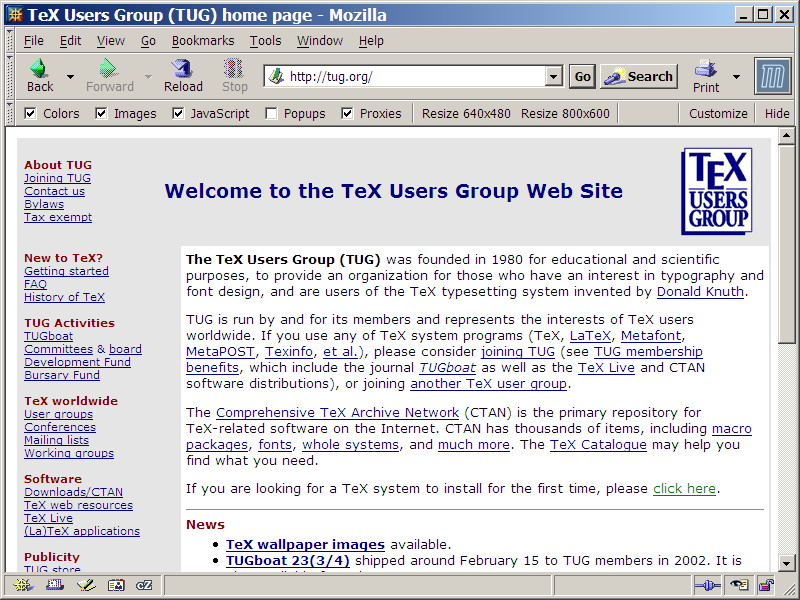
\includegraphics[keepaspectratio,width=\linewidth,height=\halfh]
{images/tugorg.png}

\caption[TeX Users Group web site]{
The web site of the TeX Users Group \parencite{TUG}.
\imgcredit{Screenshot taken by the author of this paper.}
}
\label{fig:TUG}
\end{figure}




\subsection{Installing \protect\LaTeXe}

For information about availability, versions, installation, etc. of
\LaTeXe\ consult the online
\emph{TeX Frequently Asked Questions} \parencite{TeXfaq}.
%
The best way to install \LaTeXe\ under Windows is to get the latest
TeXLive \parencite{texlive} distribution. You can download an ISO
image from CTAN TeXLive \parencite{ctan-texlive}.  Under Windows 10,
you can mount an ISO image by double-clicking, it is no longer
necessary to actually burn the image to a DVD.





\subsection{Installing Extra \protect\LaTeXe Packages}

Depending on the \LaTeXe\ package you install, you may need to install
additional or more recent versions of \LaTeXe\ packages. For example,
this thesis makes use of the \LaTeXe\ \fname{titlesec} package.
%
You can find a list of packages at your local CTAN site \parencite{CTAN}.
To install a package, read the advice at
\url{http://www.ctan.org/installationadvice/}





\subsection{Running \protect\LaTeXe}

When running \LaTeXe\ under Unix, check that the environment variables
are set to something like the values shown here:
\begin{samepage}
\begin{lstlisting}
setenv TEXINPUTS .:~/tex/inputs:./inputs::
setenv BSTINPUTS .:~/tex/inputs::
setenv BIBINPUTS .:~/tex/bib:./bib::
\end{lstlisting}
\end{samepage}


\LaTeXe\ updates certain auxiliary files during translation (for
example with figure numbers or captions) and makes use of them in
subsequent runs. To be absolutely certain that all references are
resolved correctly, run \fname{pdflatex}, \fname{biber},
\fname{pdflatex}, and \fname{pdflatex} in sequence, as shown
below for this thesis:
\begin{samepage}
\begin{lstlisting}
pdflatex thesis
biber thesis
pdflatex thesis
pdflatex thesis
\end{lstlisting}
\end{samepage}




An alternative is to use the \fname{latexmk} perl script:
\begin{samepage}
\begin{lstlisting}
latexmk --pdf thesis
\end{lstlisting}
\end{samepage}


\fname{latexmk} can also be configured using a config file such as
\lstinline|$HOME/.latexmkrc| in the user's home directory: % dummy comment $
\begin{samepage}
\begin{lstlisting}[language=Perl,]
$pdf_mode = 1;  # force use of pdflatex
\end{lstlisting}   % dummy comment $
\end{samepage}


% latexmk
% http://www.ctan.org/pkg/latexmk/
% http://users.phys.psu.edu/~collins/software/latexmk-jcc/
% http://users.phys.psu.edu/~collins/software/latexmk-jcc/latexmk-437.pdf




\subsection{Spell Checking}

GNU Aspell \parencite{Aspell} is a free open source spell checker.  It can
automatically ignore \LaTeXe\ commands. Aspell can either be run from
the command line or integrated into other packages such as Emacs.





\subsection{Integrated Development Environments (IDEs) for \protect\LaTeXe}

Under Windows you might want to use an integrated development
environment (a fancy editor) for \LaTeXe, which have built-in support
for editing \LaTeXe, spell checking, compiling, and so forth.
The IDEs assume that you have a working \LaTeXe installation,
so install \LaTeXe first.
%
The best are Texmaker \parencite{texmaker}, TeXnicCenter
\parencite{TeXnicCenter} (shown in Figure~\ref{fig:TeXnicCenter}), and LEd
\parencite{LEd}, all of which are free. The shareware WinEdt
\parencite{WinEdt} is also very good.


\begin{figure}[tp]
\centering
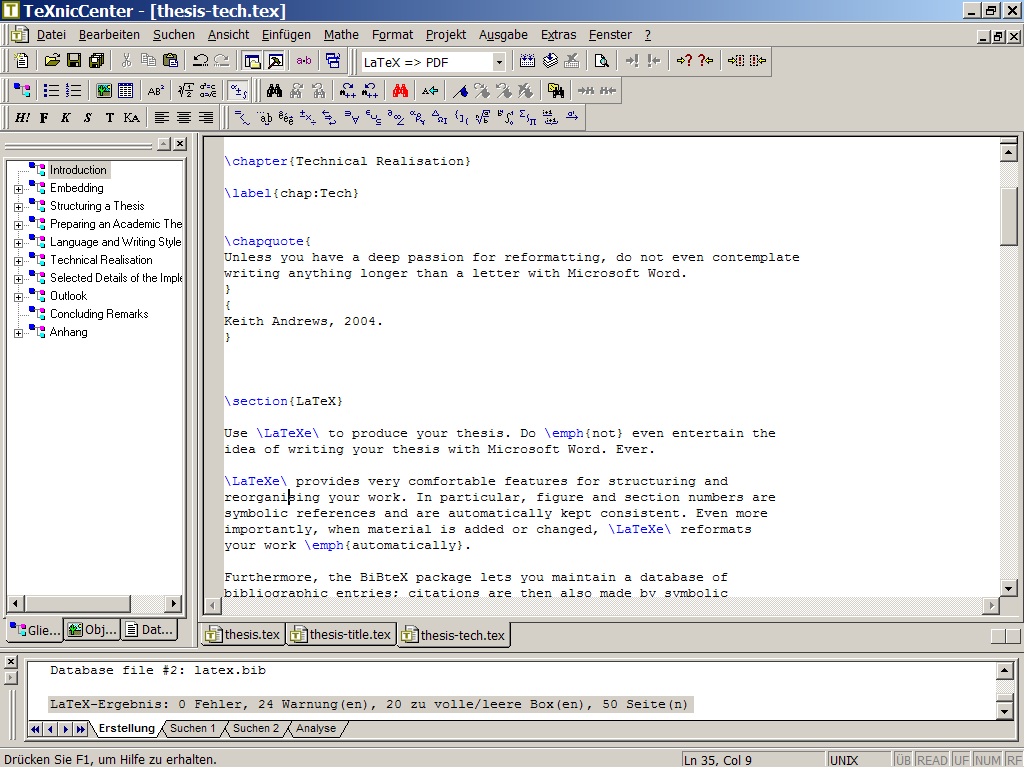
\includegraphics[keepaspectratio,width=\linewidth,height=\halfh]
{images/texnic.png}

\caption[The TeXnicCenter IDE]{
The TeXnicCenter \parencite{TeXnicCenter} integrated development
environment (IDE) for \LaTeXe.
\imgcredit{Screenshot taken by the author of this paper.}
}
\label{fig:TeXnicCenter}
\end{figure}








\section{Including Images}

Use the \fname{graphicx} package to include images.
For extra options, add the \fname{adjustbox} package:
\begin{lstlisting}
\usepackage{graphicx}
\usepackage[export]{adjustbox}    % valign=t, frame, ...
\end{lstlisting}





\subsection{Screenshots}

Screenshots are \emph{raster} images composed of pixels. Screenshots
should be made using software such as IrfanView or Gimp and always
\emph{saved as PNG}. PNG is a lossless image format which preserves
every pixel of the original image. Sometimes, novices save screenshots
as JPEG (\fname{.jpg}), which is an inherently lossy image
format. Screenshots saved as JPEG invariably introduce artefacts such
as smudged lines and text, due to the way that JPEG achieves its high
compression rates.




\subsection{Diagrams and Charts}

Diagrams and charts are most naturally expressed as \emph{vector
  graphics}, composed of graphical objects such as lines, circles,
polygons, and text strings. Vector graphics are freely scalable
without loss of quality. In contrast, \emph{raster} graphics are based
on pixels and do not scale without loss of quality. Saving diagrams
and charts in a raster format such as PNG, GIF, or JPEG means they
cannot be resized without considerable loss of quality.

Diagrams can be drawn using a vector graphics editor, such as Adobe
Illustrator \parencite{Adobe-Illustrator} or Inkscape
\parencite{Inkscape}. Make sure to archive (and hand-in) the
respective source files (\fname{.ai} or \fname{.svg}).


Charts such as line charts and bar charts can be generated by various
software packages such as R \parencite{R-Project} and gnuplot
\parencite{gnuplot}, or online tools such as Tableau \parencite{Tableau},
Flourish \parencite{Flourish}, or Datawrapper \parencite{Datawrapper}.
%
If possible, always use a tool which can save or export the chart in a
vector format, such as SVG or (vector) PDF. Many online tools,
including those above, provide vector graphics export only in their
pay-for plans.


For inclusion into \LaTeXe, the diagram or chart needs to be in vector
PDF format. If you have an SVG, you can convert it to vector PDF using
Adobe Illustrator or Inkscape. With Inkscape installed, you can use
the command line:
\begin{lstlisting}[%
  language=bash,
]
inkscape --export-type=pdf in.svg
\end{lstlisting}
or install the command-line tool CairoSVG \parencite{CairoSVG}:
\begin{lstlisting}[%
  language=bash,
]
cairosvg in.svg -o out.pdf
\end{lstlisting}


Crop the diagram or chart fairly tightly. Do not leave excessive
margins around the graphic itself, margins should be added by \LaTeXe.
Cropping can often be done in the original tool (Artboards in
Illustrator). If you have a vector PDF, it can be cropped in Acrobat
Pro (pay-for version) \parencite{Adobe-AcrobatPro} or with tools such
as briss \parencite{briss}.






\section{Including Listings}

Use the \vname{listings} package to include source code listings.
There are three types of listing:
\begin{itemize}
\item \liintro{Inline}: A small snippet of code can be contained
  within the flow of a paragraph using \lstinline!\lstinline!, for
  example \lstinline|\lstinline!var i:integer;!| produces
  \lstinline!var i:integer;!.

\item \liintro{In-Place Displayed}: An in-place displayed listing is a
  block of code listed at the place where it occurs. Use in-place
  displayed listings for short blocks of source code upto max $n$
  lines (I use $n=4$). Create an in-place displayed listing with the
  \vname{lstlisting} environment, but without using the \vname{float}
  parameter.

\item \liintro{Floating}: A floating listing is a block of code
  treated like other \LaTeXe floats (such as figures or tables). Use
  floating listings for longer blocks of code. \LaTeXe places the
  listing at some point later on. Create a floating listing with the
  \vname{lstlisting} environment, but specify the \vname{float} and
  \vname{caption} parameters. A floating listing is given a number
  (like Listing 2.1) and is listed in the List of Listings.

\end{itemize}

The \vname{listings} package is currently not designed for use with
UTF8 characters. To use UTF8 characters inside listings, you have to
specify the parameter \lstinline!inputencoding=utf8! and 
specify each character inside the \lstinline!literate=! parameter
to the \lstinline!\lstset! command.








\section{Biblatex and Biber}

BibLaTeX \parencite{BibLaTeX} is a companion system to \LaTeXe, which
allows you to manage sets of references in plain text files (called
\fname{.bib} files) and cite references from within your
\LaTeXe\ documents.  Biber \parencite{Biber} is a program which takes
\fname{.bib} files and manages the formatting of citations and of the
bibliography itself. BibLaTeX and Biber have replaced the now obsolete
BibTeX \parencite{BibTeX}.



\cleardoublepage
%----------------------------------------------------------------
%
%  File    :  survey-examples.tex
%
%  Author  :  Keith Andrews, IICM, TU Graz, Austria
% 
%  Created :  18 May 2012
% 
%  Changed :  18 May 2012
% 
%----------------------------------------------------------------

\chapter{Selected Examples of Doing Things with \LaTeXe\
(and Test of Extremely
Long Chapter Titles to See How They Work Or Not)
}

\label{chap:SelectedExamples}


This chapter contains some examples of typical \LaTeXe\
usage.




\section{Including Screenshots}

This example shows how to include a screenshot (or other raster
graphic) into a \LaTeXe\ figure. Figure~\ref{fig:Pistol} shows a VRML
model of a cavalry pistol from the Armoury in Graz displayed in the
VRwave VRML browser. Every table, figure, and listing should be
refered to from the running text.

\begin{figure}[tp]
\centering
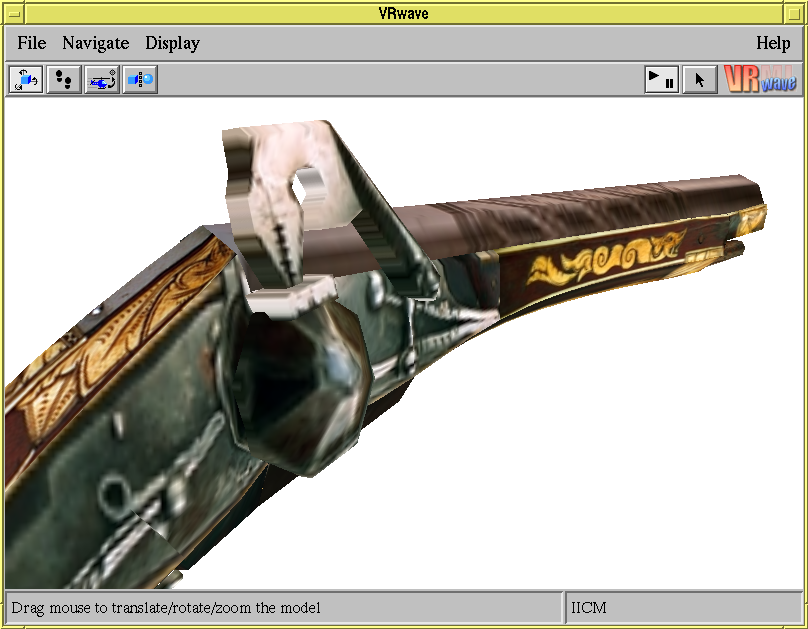
\includegraphics[keepaspectratio,width=\linewidth,height=\halfh]
{images/pist.png}

\caption[VRwave in Flip Mode]
{%
VRwave in Flip mode displaying a textured model of a cavalry pistol
from the world-renowned Zeughaus (armoury) in Graz.
\imgcredit{Image extracted from \textcite[page~81]{Andrews-VRwave}
and used under the terms of the ACM Copyright Policy. \copyrightACM}
}
\label{fig:Pistol}
\end{figure}

The caption shows an example of how to correctly cite the source when
using an image from someone else. In their 1998 paper,
\textcite{Andrews-VRwave} discuss the VRwave VRML browser.




\section{Using Subfigures}

The example in Figure~\ref{fig:RespTable} shows how to use subfigures
within a figure with the \vname{subfig} package. The figure is an
illustration of how a responsive table looks different at different
screen widths. Figure~\ref{fig:RespTableNarrow} shows the table on a
narrow screen, while Figure~\ref{fig:RespTableWide} shows the table on
a wider screen.

The source code shows usage of the \vname{includegraphics} options
\vname{frame} to draw a frame around the graphics and \vname{valign=t}
to top align them, which are both provided by the \vname{adjustbox}
package.  For this figure, it is important to ensure that both images
are scaled equally, hence the use of \vname{scale}. The exact scale
factor was determined by trial and error.


\begin{figure}[tp]
\centering
\subfloat[%  the % chars remove implicit spacing
Narrow screen.
]
{%
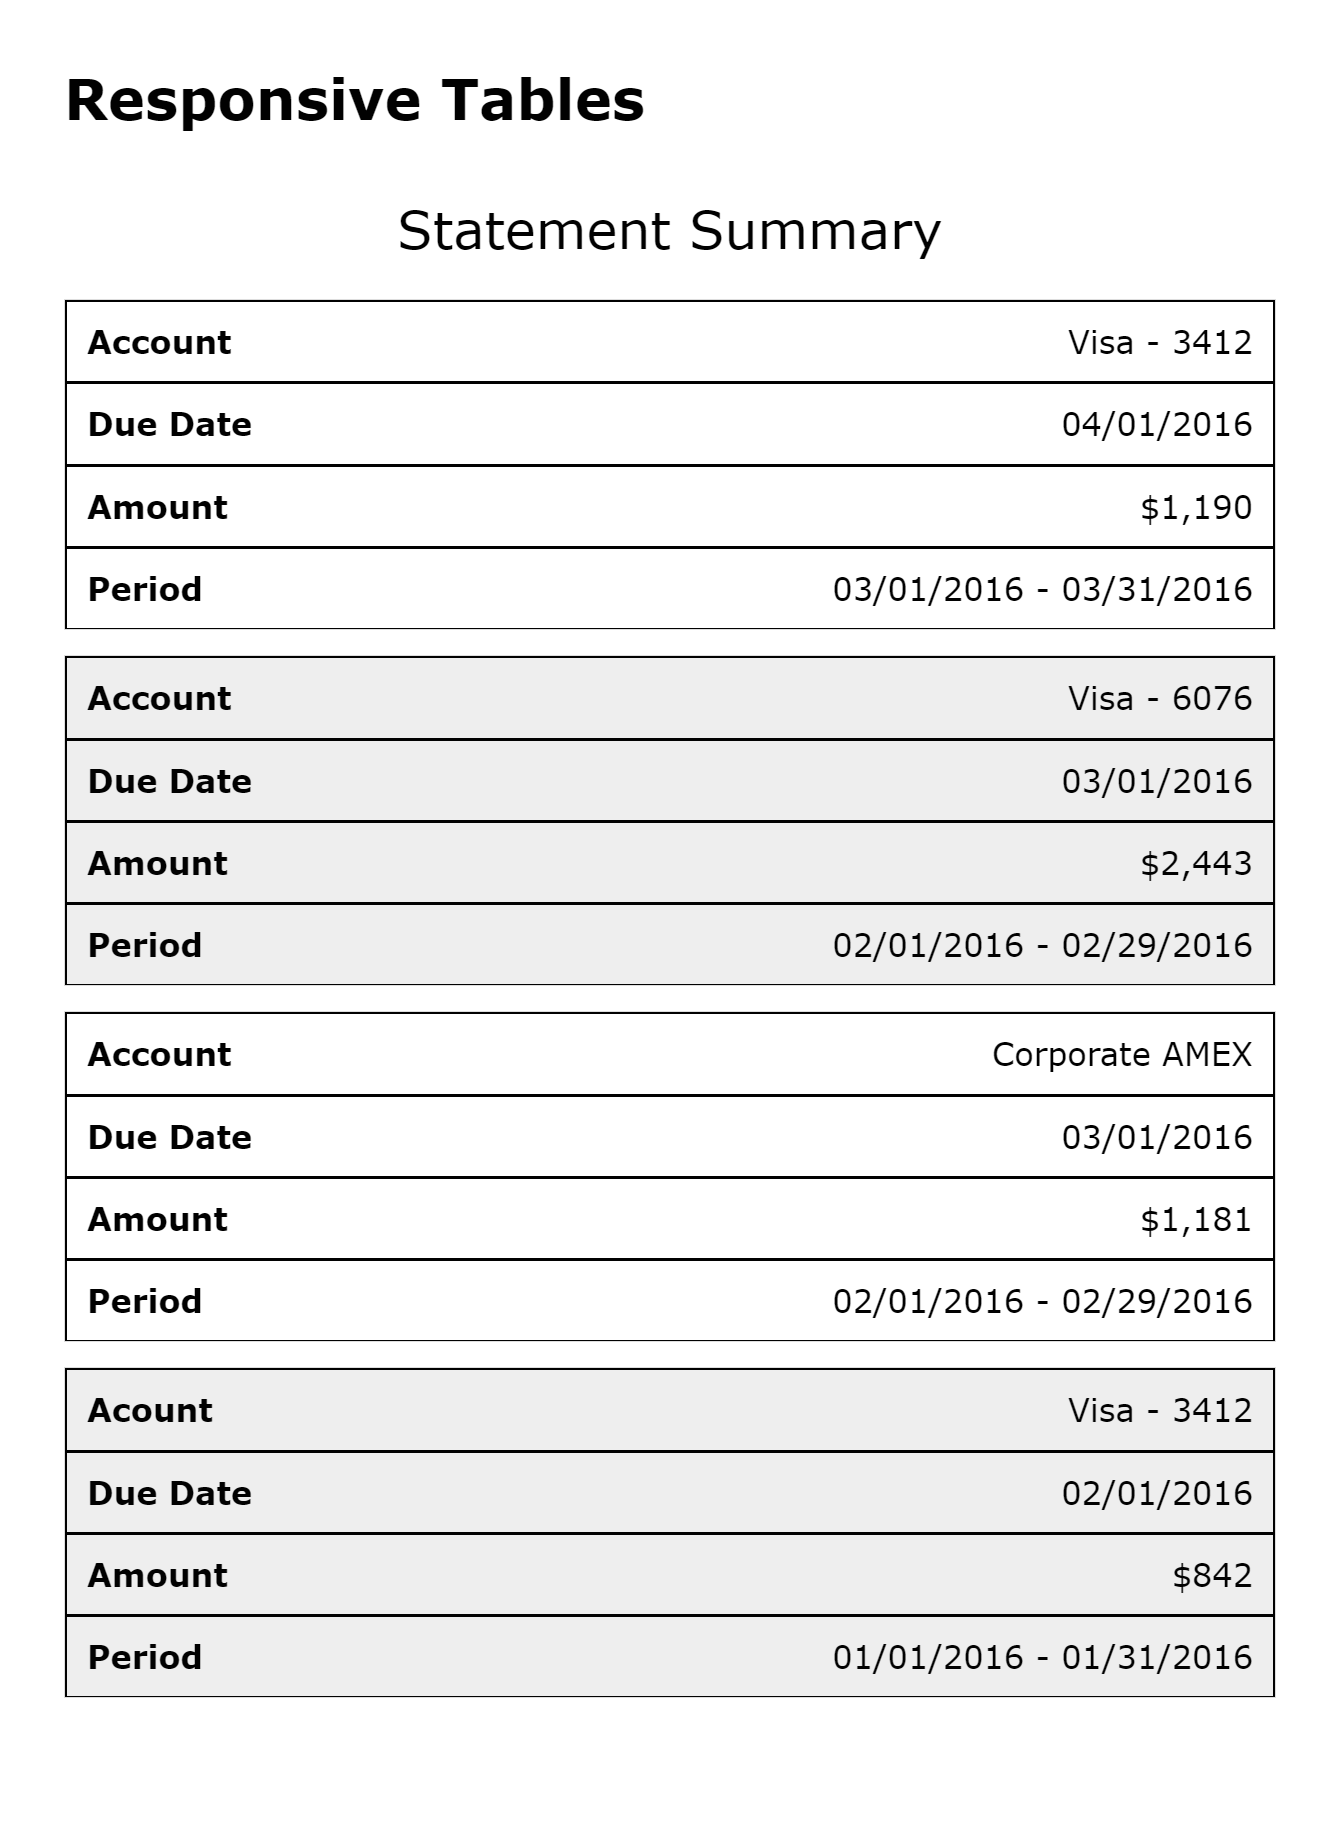
\includegraphics[valign=t,frame,scale=0.32]
{images/rt-2021-11-09-narrow-ci.png}%
\label{fig:RespTableNarrow}%
}
\hfill         % fills up the space between the two graphics
\subfloat[%
Wide ecreen.
]
{%
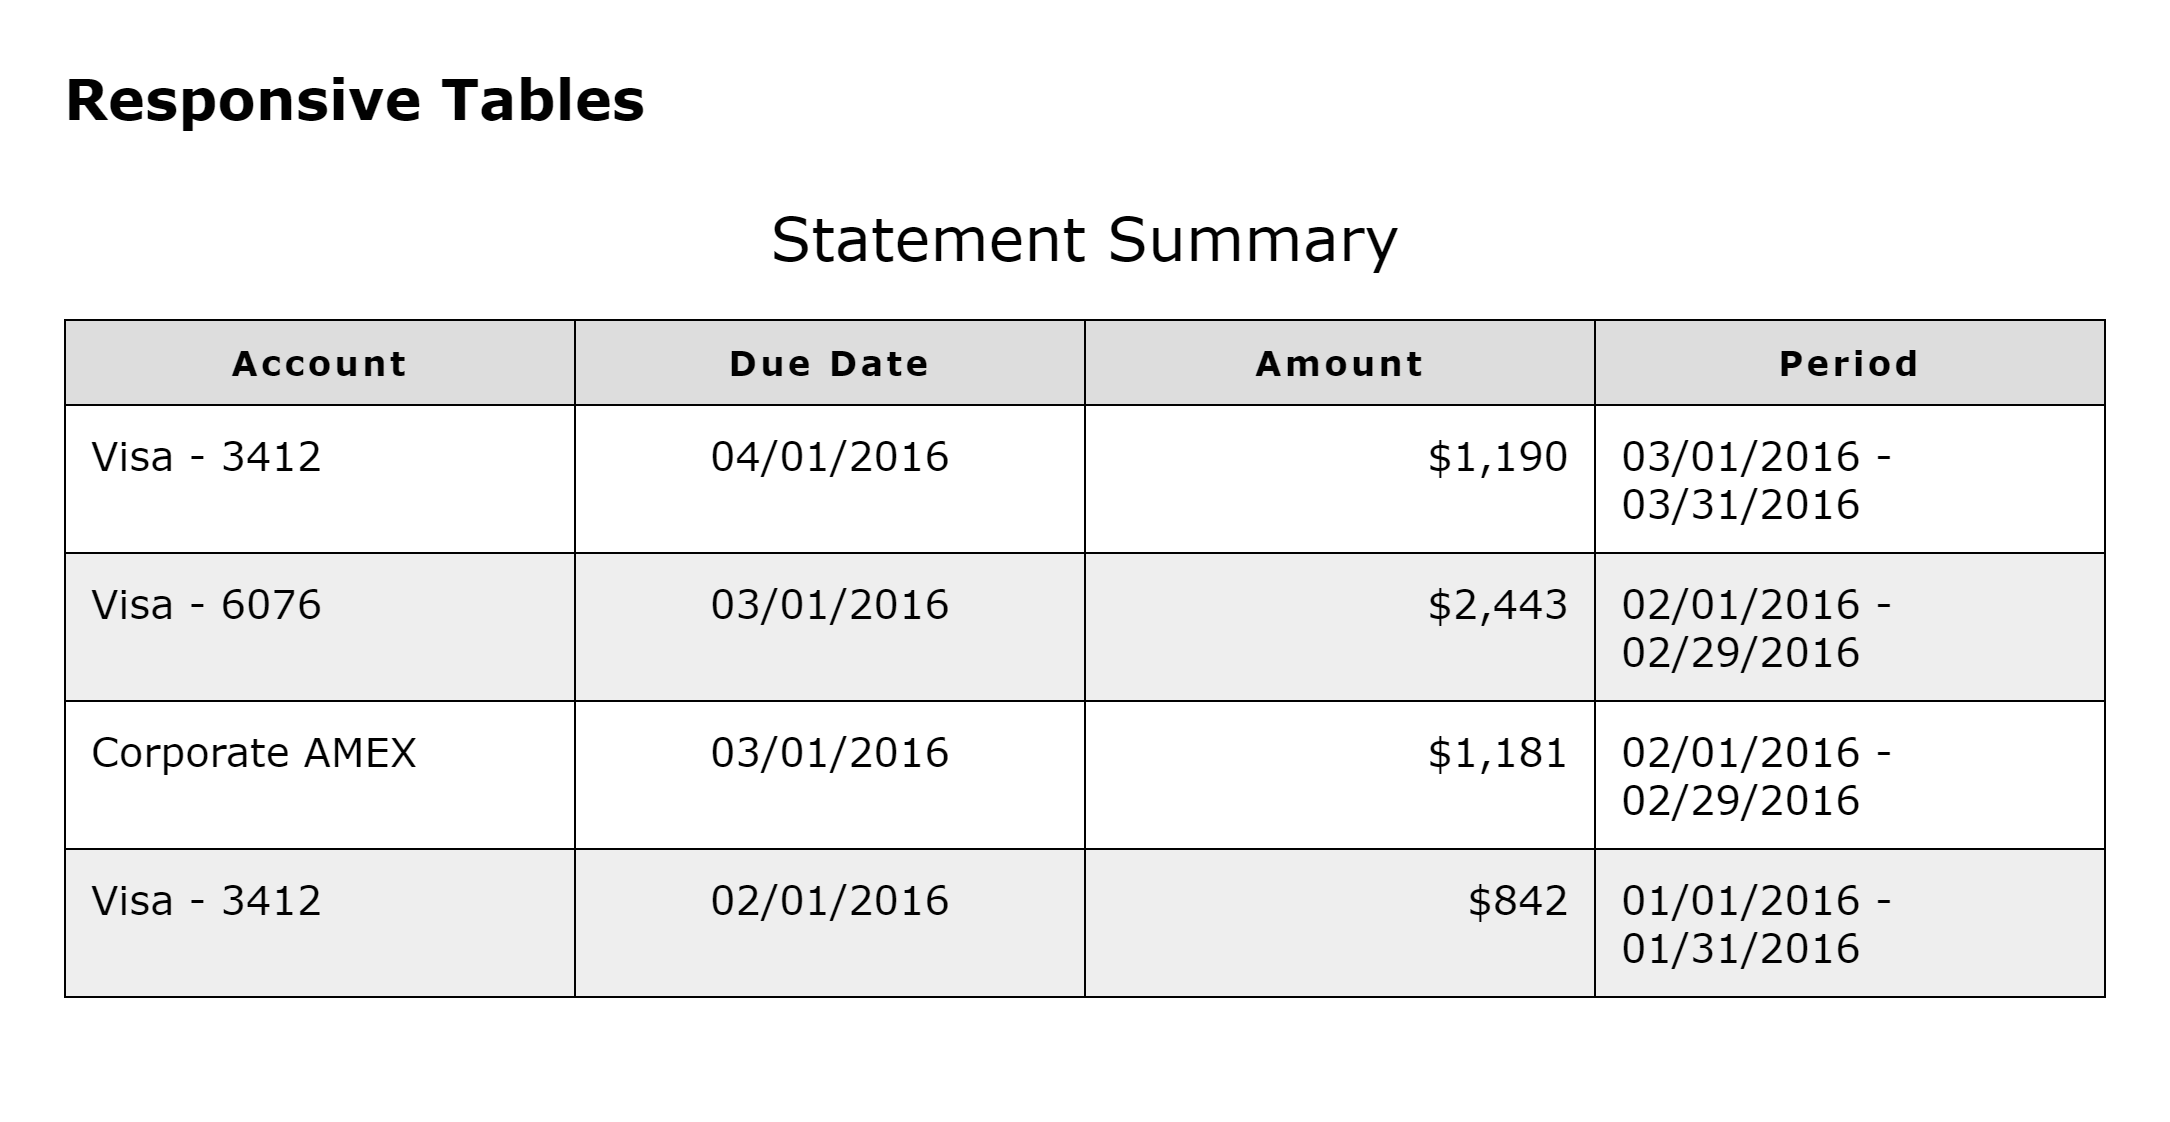
\includegraphics[valign=t,frame,scale=0.32]
{images/rt-2021-11-09-wide-ci.png}%
\label{fig:RespTableWide}%
}

\caption[Responsive Table]
{
A responsive table adapts itself to the available display space. On a
narrow screen, each row of the table is expanded vertically.
\imgcredit{Both images created by Keith Andrews.}
}
\label{fig:RespTable}
\end{figure}







\section{Including Vector Graphics}

Charts and diagrams are often naturally vector graphics, created by
assembling and arranging graphical objects such as lines, boxes,
circles, polygons, and text strings. They can usually be exported or
saved in SVG and then converted to (vector) PDF format, or saved
directly as (vector) PDF. Vector graphics have the huge benefit that
they are freely scalable: they remain crisp and sharp even when zoomed
in.
%
Vector graphics are included in LaTeX as (vector) PDF files, as shown
in Figure~\ref{fig:BreakpointDiagram}. Try zooming in to the figure in
Acrobat Reader.



\begin{figure}[tp]
\centering
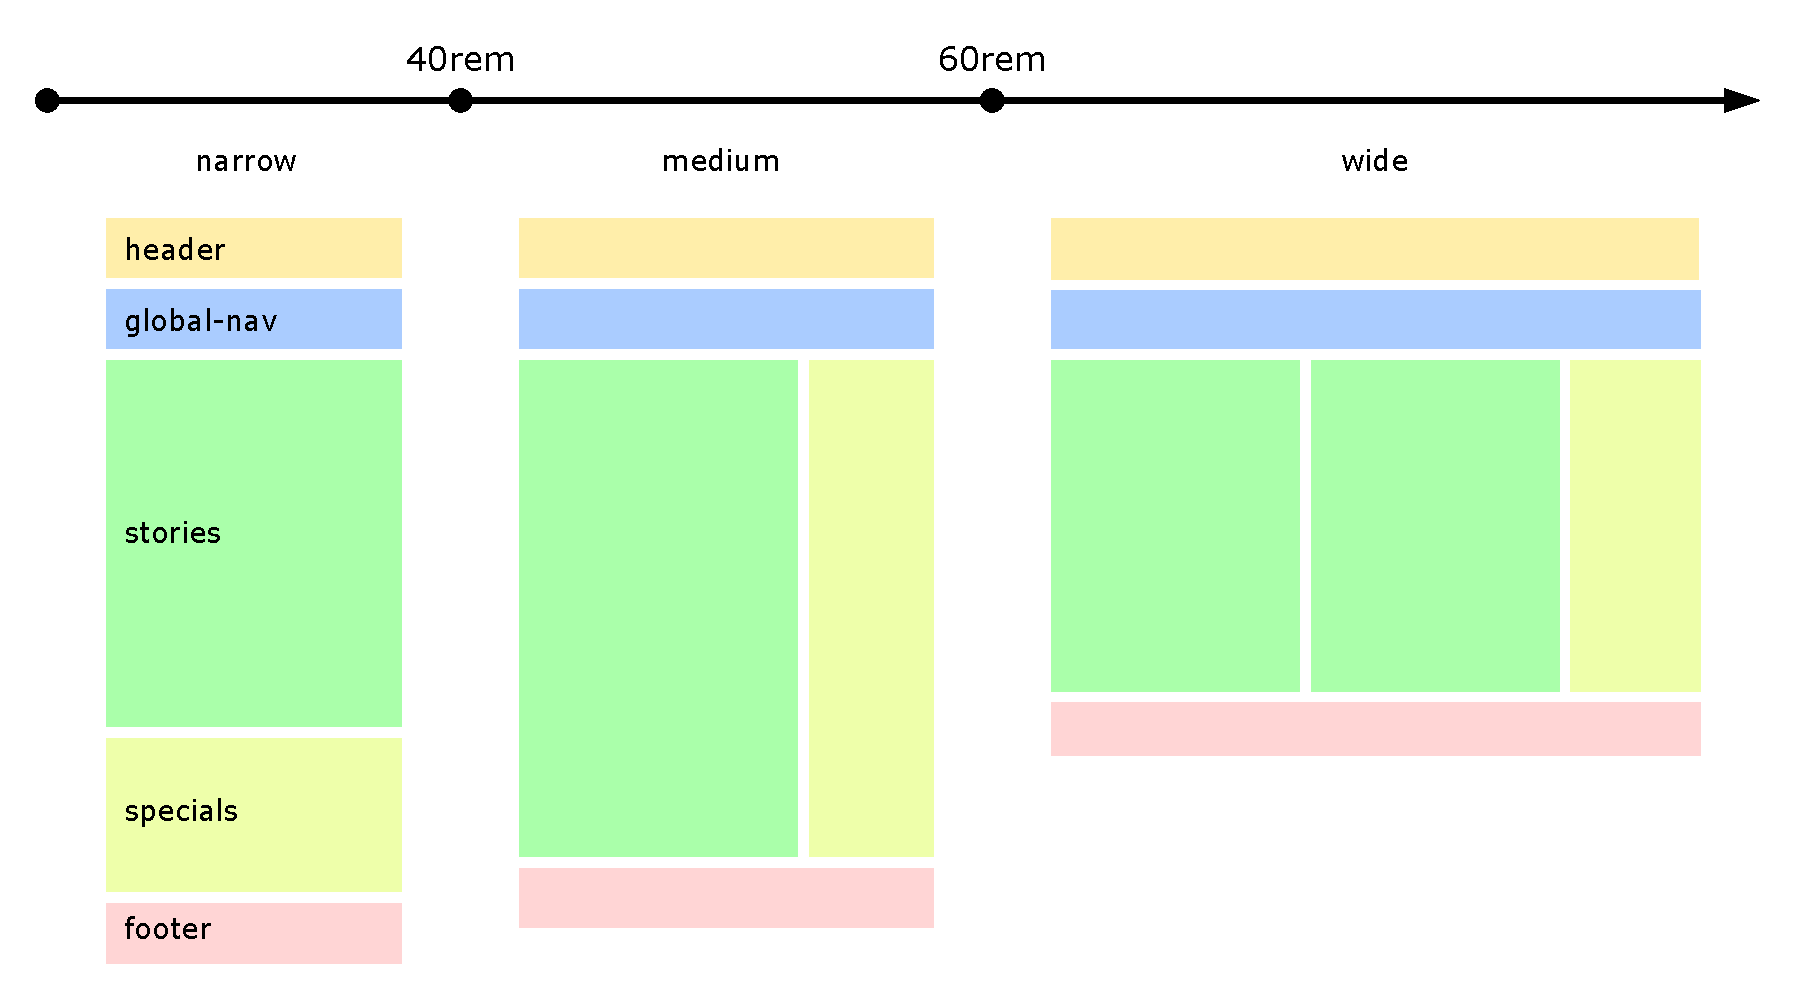
\includegraphics[frame,keepaspectratio,width=\linewidth,height=\halfh]
{diagrams/breakpoint.pdf}

\caption[Responsive Breakpoint Diagram]
{
A responsive breakpoint diagram. Setting breakpoints at 40 rem and 60 rem
provides for three different layouts: narrow, medium, and wide.
The layout scales smoothly between breakpoints and changes at a breakpoint.
\imgcredit{Drawn by Keith Andrews.}
}
\label{fig:BreakpointDiagram}
\end{figure}










\section{Using Tables}

An example of using a table can be seen in Table~\ref{tab:SomePubs}.

\begin{table}[tp]
\tablestretch
\rowcolors{2}{}{tablerowcolour}
\centering
\begin{tabularx}{\linewidth}
{>{\kern-\tabcolsep}lllX<{\kern-\tabcolsep}}
\toprule
\textbf{Name} & \textbf{Type} & \textbf{Rating} & \textbf{Description} \\
\midrule
Flann O'Brien & Irish / International & ***** &
In the centre of town, easy for
marauding tourists to find. Good food, smooth Guinness.\\
%
Dublin Road & Irish & ***** &
In the old town, best Guinness in Graz.
Regular live music. Irish session every Wednesday.\\
%
O'Carolan's & Irish & **** &
In the centre of town in a small side street next to Flann's.
Small, cosy, open late.\\
%
Two Brothers & Irish / English & **** &
Hidden in the narrow streets of the old town.
Erasmus student night on Wednesday.\\
%
O'Sullivan's & Irish / Austrian & **** &
Cosy, friendly place, many regulars.\\
%
O'Riginal & Austrian & ** &
Near to Jakominiplatz.
Small place with Guinness. Regular live music.\\
\bottomrule
\end{tabularx}

\caption[Some Pubs in Graz]
{
Some pubs in Graz.
}
\label{tab:SomePubs}
\end{table}









\section{Using Special Characters and Symbols}

You can use many (but not all) of the thousands of characters
available in the UTF-8 \parencites{Wikipedia-UTF8}{Unicode-Charts}
character encoding. For example, the German umlauts (äüö), the German
sharp s (ß), or the yen symbol (¥).

You can also try some of the \approxsym 100 symbols available
in the \vname{textcomp} package, such as the yen symbol (\textyen) and
a circled letter A (\textcircled{A}).





\section{Using Macros to Style Special Names}

Sometimes, a macro (new command definition) can be useful to style
special names or phrases consistently. For example, if you are often
refering to named components of a user interface, such as the
\uiname{Toolbar} or \uiname{Status Panel}, then define a macro
\verb|uiname|, so that all such components can be styled consitently:
\begin{lstlisting}
\newrobustcmd{\uiname}[1]{{\smaller\textsf{#1}}}
\end{lstlisting}

Macros like \vname{vname}, \vname{cname}, and \vname{fname} can be
used to style (say) variable names, class names, and file names. This
is a long file name
\fname{/usr/data/keith/travel/austria/vienna.txt}. This is a typical
class name in camel case \cname{HVSInformationPyramidsInputFactory}.





\section{Using Floating Listings}

Listing~\ref{list:HTML5Boilerplate} is floating. A floating listing is
a block of code treated like other \LaTeXe floats (such as figures or
tables). Use floating listings for longer blocks of code.
A floating listing is given a number and can be referred to
explicitly, like Listing~\ref{list:HTML5Boilerplate}. It can be given
a caption and short caption, and is listed in the List of Listings.


\begin{samepage}
\begin{lstlisting}[%
  float=tp,
  aboveskip=\floatsep,
  belowskip=\floatsep,
  xleftmargin=0cm,              % no extra margins for floats
  xrightmargin=0cm,             % no extra margins for floats
  language=HTML,
  basicstyle=\footnotesize\ttfamily,
  frame=shadowbox,
  numbers=left,
  label=list:HTML5Boilerplate,
  caption={[HTML5 Boilerplate Code]%
Some HTML5 boilerplate code, illustrating the typical structure
of a HTML5 web page.
},
]
<!DOCTYPE html>
<html xmlns="http://www.w3.org/1999/xhtml" lang="en" xml:lang="en">

<head>
<meta charset="UTF-8"/>
<meta name="viewport" content="width=device-width, initial-scale=1"/>
<link rel="stylesheet" href="./inm.css"/>

<title>Keith Andrews Web Page</title>
</head>

<body>

<header>
<img src="images/kalogo.svg" alt="KA Logo"/>
Keith Andrews Design
</header>

<h1>Keith Andrews</h1>

<p>
Keith lives in <a href="http://graz.at/">Graz</a>.
</p>

<p>
<img src="images/keith-s.jpg"
  alt="Photo of Keith Andrews"/>
</p>

<p>
Three desirable attributes:
</p>
<ol>
<li>cheap</li>
<li>fast</li>
<li>good</li>
</ol>
<p>
Choose any two.
</p>

<p>
<abbr title="Extensible HyperText Markup Language">XHTML</abbr>
is cool.
</p>

<table>
<tbody>
<tr><th>Beer</th><th>Price €</th></tr>
<tr><td>Puntigamer</td><td>2,60</td></tr>
<tr><td>Gösser</td><td>2,60</td></tr>
<tr><td>Guinness</td><td>4,35</td></tr>
</tbody>
</table>

<footer>
Copyright © Keith Andrews 2019.
</footer>

</body>
</html>
\end{lstlisting}
\end{samepage}










\section{Using Non-Floating Diplayed Listings}

The listing below shows some CSS:
\begin{samepage}
\begin{lstlisting}[%
  language=CSS,
]
body { color: black; background-color: silver; }
img { border: none; }
h1,h2 { font-family: Verdana, sans-serif; }
\end{lstlisting}
\end{samepage}
It is displayed (i.e. indented as a block) in-place, but is not
floating. It cannot be referred to by number and is not listed in the
List of Listings. As a rule of thumb, if listings have five or more
lines, make them floating.





\section{Using Inline Listings}

Inline listings are used for very short snippets of code embedded
within the flow of a paragraph. For example,
\lstinline|\lstinline!var i:integer;!|
produces
\lstinline!var i:integer;!, which can now be discussed further.
Do not break an inline listing over multiple lines (EOL).




\section{Using Lists}

A list should always be introduced by a sentence
which ends with a colon.
%
There are three kinds of standard lists in \LaTeXe:
\begin{itemize}
\item itemize
\item enumerate
\item description
\end{itemize}
% A blank line here would indicate a new (indented) paragraph
An enumerated list has numbered items:
\begin{enumerate}
\item Fast
\item Good
\item Cheap
\end{enumerate}
Choose any two!


A description list has named items with corresponding
definitions or descriptions:
\begin{description}
\item[Short] Each item has a label (name) and its description.

\item[Rather longer label] By default, if the description text
  is rather long, it will warp around to the following lines.
\end{description}



\cleardoublepage
%----------------------------------------------------------------
%
%  File    :  survey-concl.tex
%
%  Author  :  Keith Andrews, IICM, TU Graz, Austria
% 
%  Created :  27 May 1993
% 
%  Changed :  16 Nov 2010
% 
%----------------------------------------------------------------


\chapter{Concluding Remarks}

\label{chap:Concl}



At the end of your survey, give a clear recommendation
as to which approach or tool to use in which situation.





\cleardoublepage
% for now, switch to language english
% hack to force unix date for biblio, biblatex 3.11
\begin{otherlanguage}{english}
\printbibliography[heading=bibintoc]
\end{otherlanguage}


\end{document}

